\documentclass[a0,portrait,final]{baposter_old}

\usepackage[utf8]{inputenc}

\tracingstats=2

%\usepackage{lipsum}
\usepackage{graphicx}

\usepackage{times}
\usepackage{calc}
%\usepackage{graphicx}
\usepackage{amsmath}
\usepackage{amssymb}
\usepackage{relsize}
%\usepackage{multirow}
\usepackage{bm}
\usepackage{graphicx}
\usepackage{multicol}
%\usepackage{pgfbaselayers}
\pgfdeclarelayer{background}
\pgfdeclarelayer{foreground}
\pgfsetlayers{background,main,foreground}
\usepackage{helvet}
%\usepackage{bookman}
\usepackage{palatino}
\newcommand{\captionfont}{\footnotesize}
\selectcolormodel{cmyk}
\graphicspath{{images/}}

% Some math symbols used in the text
\newcommand{\Matrix}[1]{\begin{bmatrix} #1 \end{bmatrix}}
\newcommand{\Vector}[1]{\Matrix{#1}}
\newcommand*{\SET}[1]  {\ensuremath{\mathcal{#1}}}
\newcommand*{\MAT}[1]  {\ensuremath{\mathbf{#1}}}
\newcommand*{\VEC}[1]  {\ensuremath{\bm{#1}}}
\newcommand*{\CONST}[1]{\ensuremath{\mathit{#1}}}
\newcommand*{\norm}[1]{\mathopen\| #1 \mathclose\|}% use instead of $\|x\|$
\newcommand*{\abs}[1]{\mathopen| #1 \mathclose|}% use instead of $\|x\|$
\newcommand*{\absLR}[1]{\left| #1 \right|}% use instead of $\|x\|$
\def\norm#1{\mathopen\| #1 \mathclose\|}% use instead of $\|x\|$
\newcommand{\normLR}[1]{\left\| #1 \right\|}% use instead of $\|x\|$

%Author's defs
\def\afi#1{$^{(#1)}$}
\def\bu{\textcolor{red}{\textbullet~}}
%---------- Author's commands---------------------------------
%\def\rsun{R$_{\rm SUN}$}
\def\bA{{\bf A}}
\def\ba{{\boldsymbol{a}}}
\def\bB{{\bf B}}
\def\bb{{\bf b}}
\def\bC{{\bf C}}
\newcommand{\dd}{\mathrm{d}}
\def\bD{{\bf D}}
\def\bd{{\bf d}}
\def\be{{\boldsymbol{e}}}
\def\bF{{\bf F}}
\def\bff{{\bf f}}
\def\bg{{\bf g}}
\def\bG{{\bf G}}
\def\bh{{\bf h}}
\def\bH{{\bf H}}
\def\bi{{\bf i}}
\def\bI{{\boldsymbol{I}}}
\def\bk{{\bf k}}
\def\bK{{\bf K}}
\def\bM{{\bf M}}
\def\bn{{\boldsymbol{n}}}
\def\boo{{\boldsymbol{o}}}
\def\bp{{\boldsymbol{p}}}
\def\bP{{\bf $P$}}
\def\bq{{\boldsymbol{q}}}
\def\bQ{{\bf Q}}
\def\br{{\boldsymbol{r}}}
\def\bR{{\bf R}}
\def\bs{{\bf s}}
\def\bS{{\bf S}}
\def\bt{{\bf t}}
\def\bT{{\bf T}}
\def\bU{{\bf U}}
\def\bW{{\bf W}}
\def\bx{{\bf x}}
\def\by{{\bf y}}
\def\bSigma{{\bf \Sigma}}
\def\bLambda{{\bf \Lambda}}
\def\blambda{{\bf \lambda}}
\def\bN{{\bf \mathcal{N}}}
\def\bchi{\boldsymbol{\chi}}
\def\bxi{\boldsymbol{\xi}}
\def\bzeta{\boldsymbol{ \zeta}}
\newcommand{\lbl}{\mbox{\boldmath $\hat{l}$}}
\newcommand{\lpl}{\mbox{\boldmath $\hat{p}$}}
\def\deg{$^\circ$}
\def\mdeg{^\circ}
\def\bbp{{\bf p}}

\def\rsun{R$_\odot$}
\def\deg{$^\circ$}
\def\mdeg{^\circ}
%\def\tr{\textcolor{blue}{$\blacktriangleright$~}}
\def\bu{\textcolor{red}{\textbullet~}}
\def\tr{\bu}
\def\bbu{\textbullet~}
\def\cmsq{cm$^2$}
\def\cmcu{cm$^3$}
\def\azul#1{\textcolor{blue}{\bf\sf #1}}
\def\eazul#1{\textcolor{blue}{\emph{#1}}}
\def\rojo#1{\textcolor{red}{#1}}

\def\verde#1{\textcolor{green}{#1}}
\def\orange#1{\textcolor{orange}{#1}}
\def\bL{{\bf L}}
\newcommand{\DT}{\Delta T}


\def\bazul#1{\textcolor{blue}{\bf\tt #1}}
\def\brojo#1{\textcolor{red}{\bf\tt #1}}

\def\ldem{{\sf LDEM}}

\def\saltito{\vskip 0.1cm}
\def\saltito{\vskip 0.1cm}

\newcommand{\mrsun}{\rm{R}_\odot}
\newcommand{\mAU}{\rm{AU}}
\newcommand{\mhr}{\rm{hr}}

\def\Ne{\rm{N_e}}
\def\Eeuv{E_{\rm{EUV}}}
\def\Ewl{E_{\rm{WL}}}
\def\AvgNeSQ{\left< N_e^2 \right>}
\def\AvgNe{\left< N_e \right>}
\def\SigmaNe{\sigma_{Ne}}
\def\VarNe{\rm{Var}N_e}
\def\AvgTe{\left<T_e\right>}
\def\SigmaTe{\sigma_{Te}}
\def\AFe{[\rm{Fe}]}

%----------------------------------------------------------------------
% From Rich's Note:
\def\bc{{\bf c}}
\def\rd{\mathrm{d}}  
\def\by{\boldsymbol{y}}
\def\bepsilon{\boldsymbol{\epsilon}}
\def\bSigma{{\bf \Sigma}}
\def\rT{\mathrm{T}}

%----------------------------------------------------------------------

% Multicol Settings
\setlength{\columnsep}{0.2em}
\setlength{\columnseprule}{0mm}

% Save space in lists. Use this after the opening of the list
\newcommand{\compresslist}{%
\setlength{\itemsep}{1pt}%
\setlength{\parskip}{0pt}%
\setlength{\parsep}{0pt}%
}

% Begin of Document
\begin{document}

% Here starts the poster
% Format it to your taste with the options
% Define some colors
\definecolor{silver}{cmyk}{0,0,0,0.3}
\definecolor{yellow}{cmyk}{0,0,0.9,0.0}
\definecolor{reddishyellow}{cmyk}{0,0.22,1.0,0.0}
\definecolor{black}{cmyk}{0,0,0.0,1.0}
\definecolor{darkYellow}{cmyk}{0,0,1.0,0.5}
\definecolor{darkSilver}{cmyk}{0,0,0,0.1}
\definecolor{lightyellow}{cmyk}{0,0,0.3,0.0}
\definecolor{lighteryellow}{cmyk}{0,0,0.1,0.0}
\definecolor{lighteryellow}{cmyk}{0,0,0.1,0.0}
%\definecolor{lightestyellow}{cmyk}{0,0,0.05,0.0}
\definecolor{MyLightMagenta}{cmyk}{0.1,0.8,0,0.1}
%\definecolor{MyDarkBlue}{rgb}{0.1,0,0.55} 
%\definecolor{MyLightBlue}{rgb}{0.1,0,0.1} 

\definecolor{MyDarkBlue}{cmyk}{1,0.7,0.4,0}
\definecolor{MyLightBlue}{cmyk}{0.2,0.05,0.1,0}
\definecolor{light-gray}{gray}{0.85}
\definecolor{light-gray2}{gray}{0.65}
%%



\typeout{Poster Starts}

\background{
\begin{tikzpicture}[remember picture,overlay]
\draw (current page.north west)+(-2em,2em) node[anchor=north west]{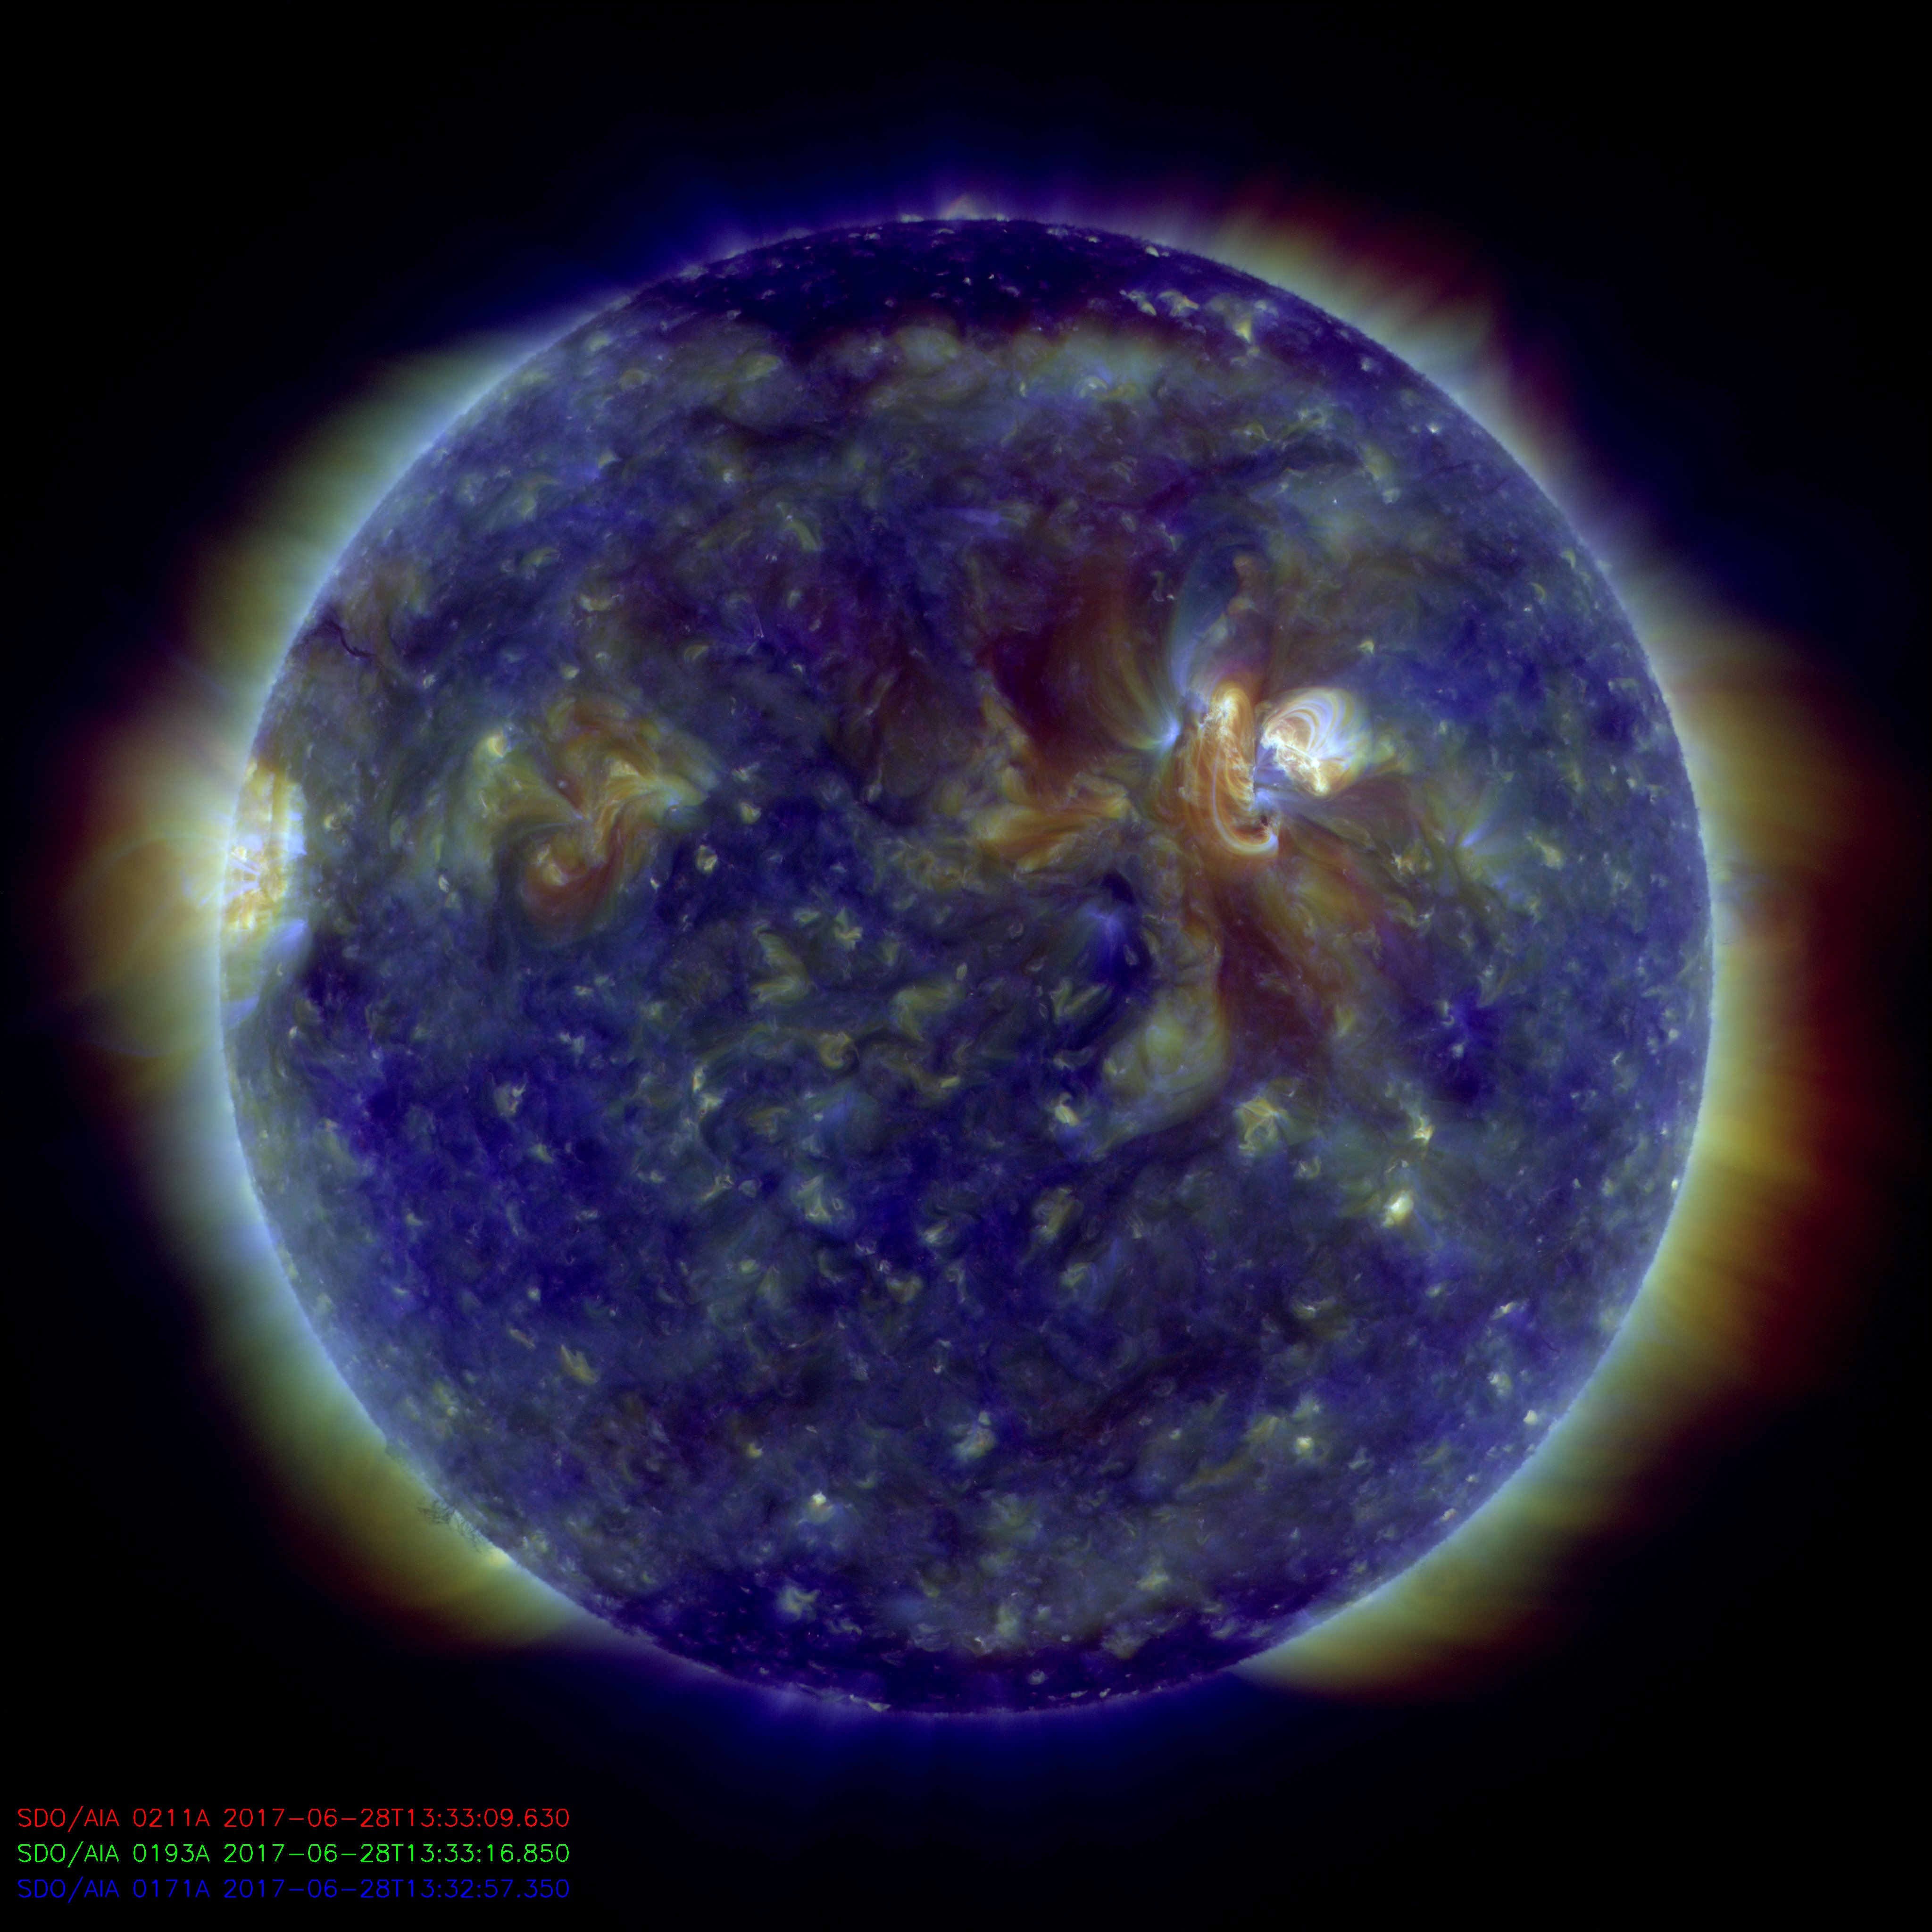
\includegraphics[width=1.1\paperheight,height=1.1\paperheight]{AIA.jpg}};
  \end{tikzpicture}
}

\newlength{\leftimgwidth}
\begin{poster}%
  % Poster Options
  {
  % Show grid to help with alignment
  grid=no,
  % Column spacing
  colspacing=1em,
  % Color style
  bgColorOne=MyLightBlue,%lighteryellow,
  bgColorTwo=MyLightBlue,%lightestyellow,
  borderColor=MyDarkBlue,%reddishyellow,
  headerColorOne=MyDarkBlue,
  headerColorTwo=reddishyellow,
  headerFontColor=white,
  boxColorOne=MyLightBlue,
  boxColorTwo=MyLightBlue,
  % Format of textbox
  textborder=roundedleft,
  % Format of text header
  eyecatcher=yes,
  headerborder=open,
  headerheight=0.05\textheight,
  headershape=roundedright,
  headershade=plain,
  headerfont=\large\sf, %Sans Serif
  boxshade=plain,
%background=shade-tb,
  background=plain,
  background=user,
  linewidth=1pt
  }
  {\setlength\fboxsep{0pt}\setlength\fboxrule{0.5pt}
  \fbox{
\includegraphics[height=5.em]{logo_IAFE.pdf}}}
 % Title
 {\sf\textcolor{white}%{MyDarkBlue}
 {\vskip 0.25cm \bf \Large Towards Multi Instrument Tomography of the Solar Corona}}
% Authors
{\footnotesize\sf
\textcolor{white}{Diego G. Lloveras\afi{1}{\bf\tt(dlloveras@iafe.uba.ar)}, Alberto M. Vásquez\afi{1}{\bf\tt(albert@iafe.uba.ar)}, Enrico Landi\afi{2} and Richard A. Frazin\afi{2}  
\vskip 0.1cm
\afi{1}Instituto de Astronom\'\i a y F\'\i sica del Espacio, CONICET--UBA, Argentina.
\vskip 0.05cm
\afi{2}Department of Climate and Space Sciences and Engineering, University
of Michigan, EEUU}}
{\setlength\fboxsep{0pt}\setlength\fboxrule{0.5pt}
\fbox{
\includegraphics[height=5.em]{logo_CLASP.pdf}}}


\headerbox{\centerline{Abstract}}{name=abstract,column=0,row=0,span=3}{
\begin{center} 
{\footnotesize\sf
\azul{Solar rotational tomography (SRT)} allows reconstruction of the three-dimensional (3D) distribution of the coronal electron density $N_e$. Using white light images the electron density results are of an absolute nature. Using Extreme Ultraviolet (EUV) images the results depend on the iron coronal abundance [Fe] and the coronal density irregularity factor $X\equiv\left<N_e^2\right>/\left<N_e\right>^2$, where $\left<\right>$ indicates the average over the tomographic voxel. Applying both methodologies independently allows determination of $X$ assuming values for [Fe]. We develop a new tomographic technique that jointly exploits optical and EUV data, that will allow determination of these parameters in a joint manner along with other fundamental coronal parameters. In this work we describe the technique, dubbed \azul{Multi Instrument Tomography}, currently under development.

}
\end{center}
}

\headerbox{What is Solar Rotational Tomography?}{name=Tom,column=0,below=abstract,span=3}{
{\footnotesize\sf
{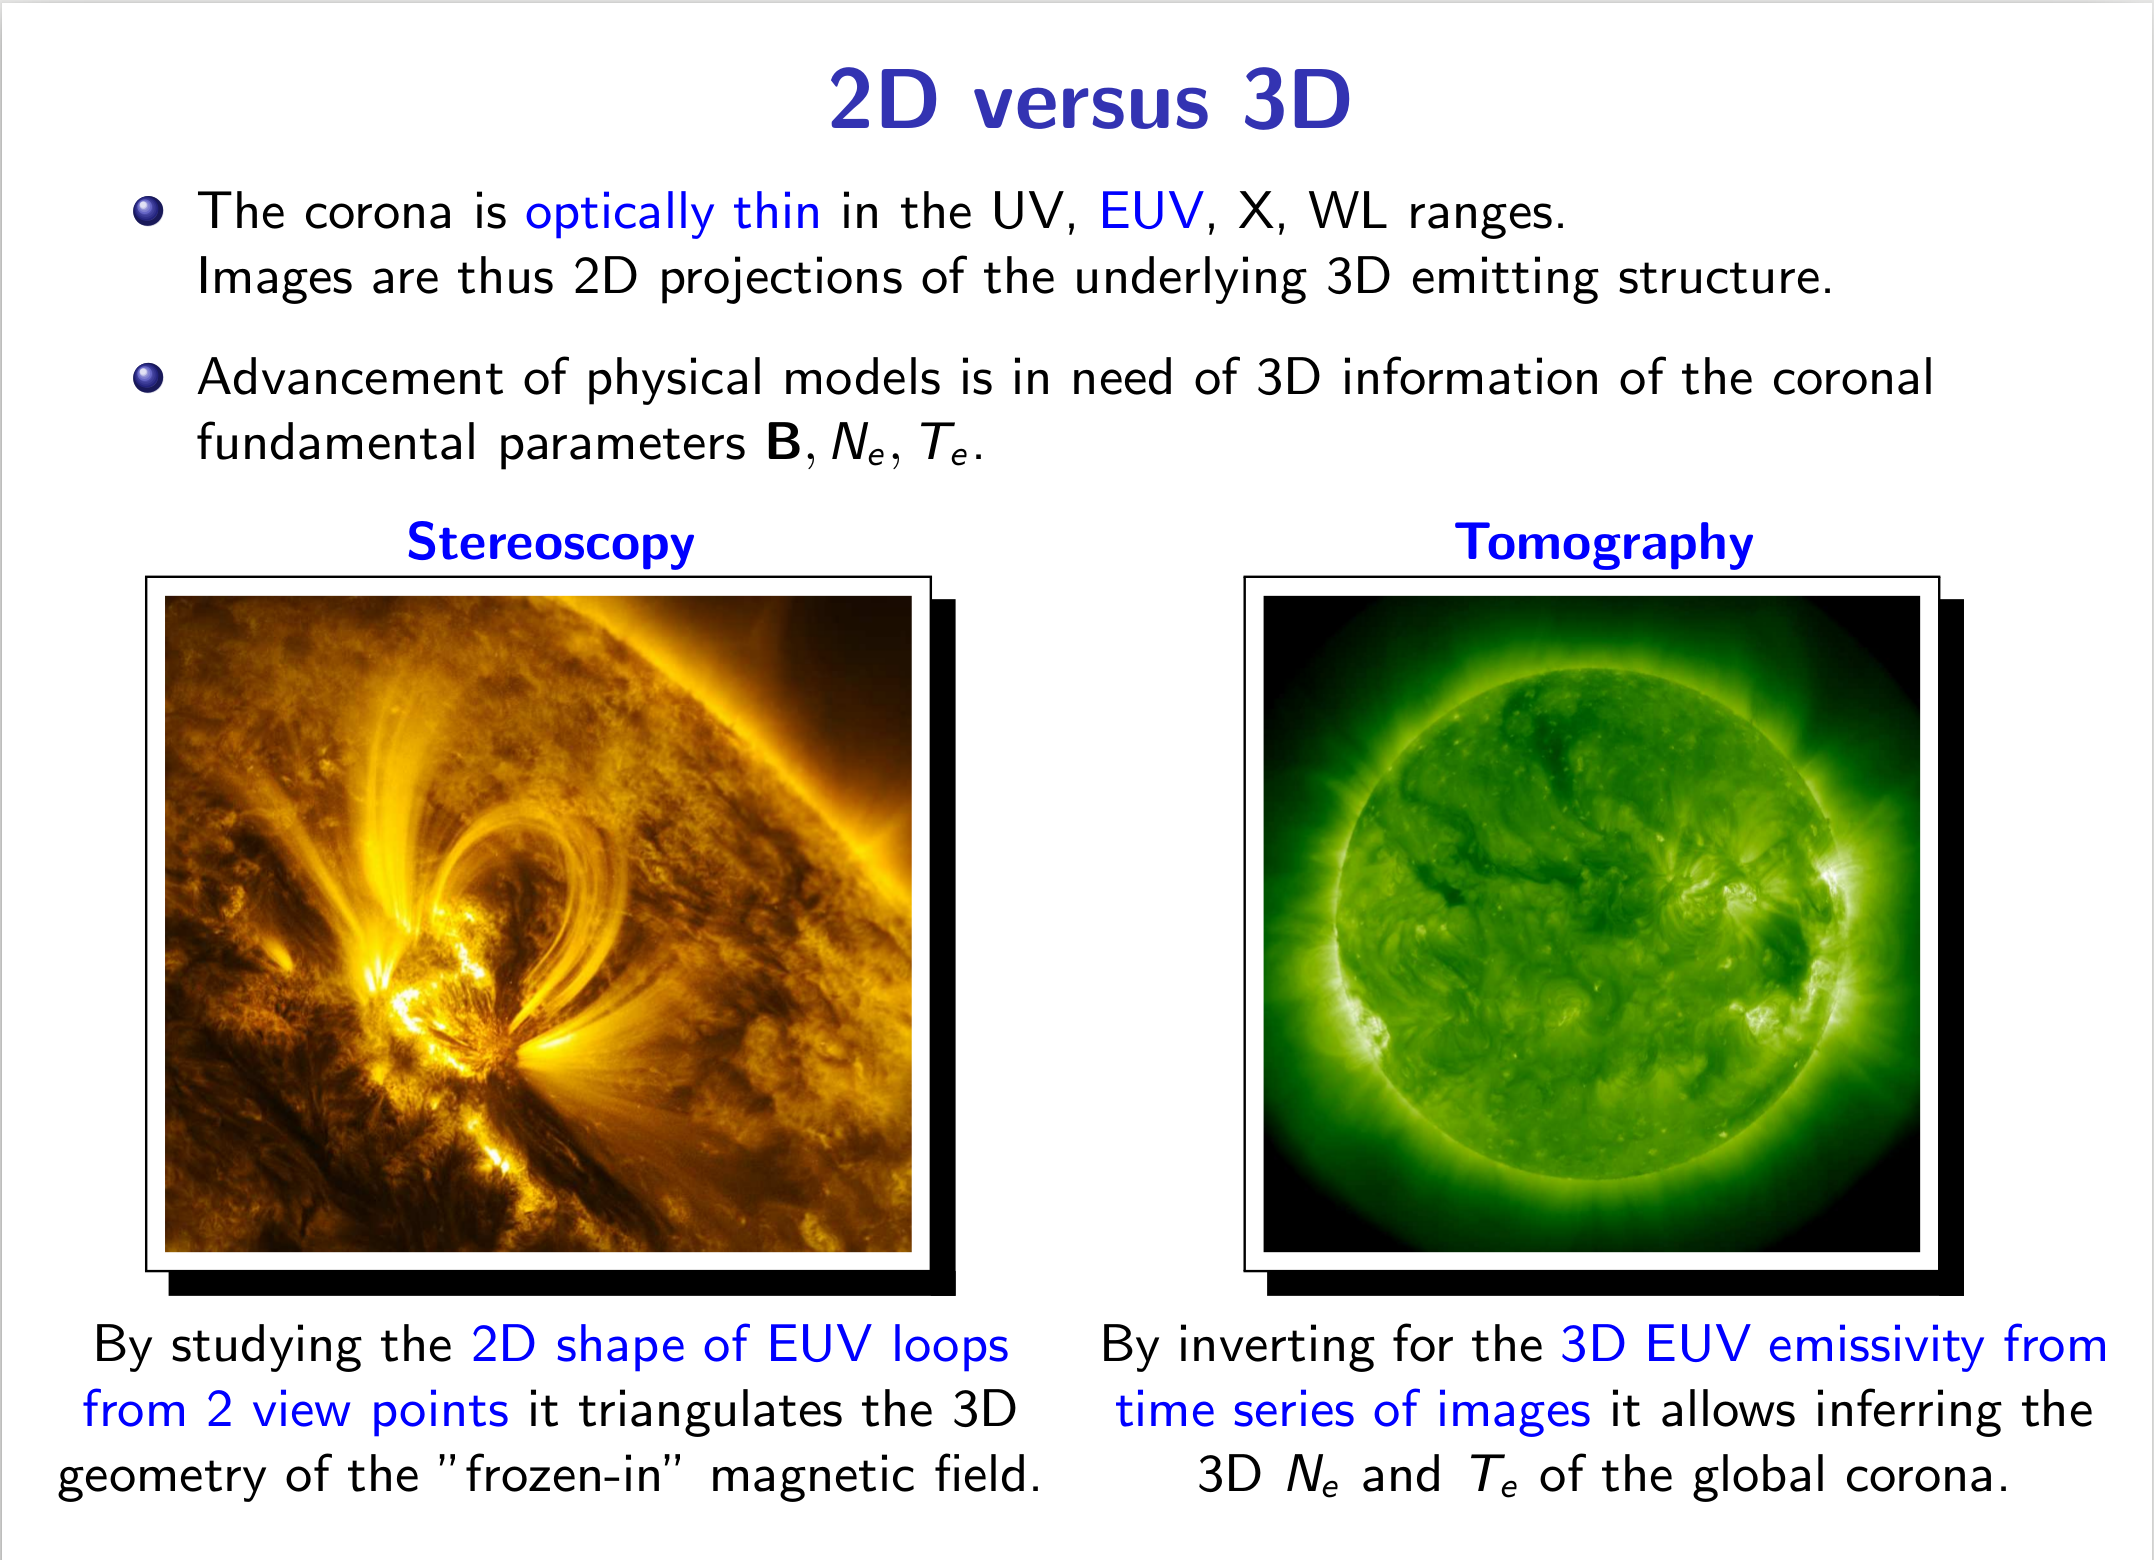
\includegraphics[width=0.33\textwidth]{tomo1.png}}
{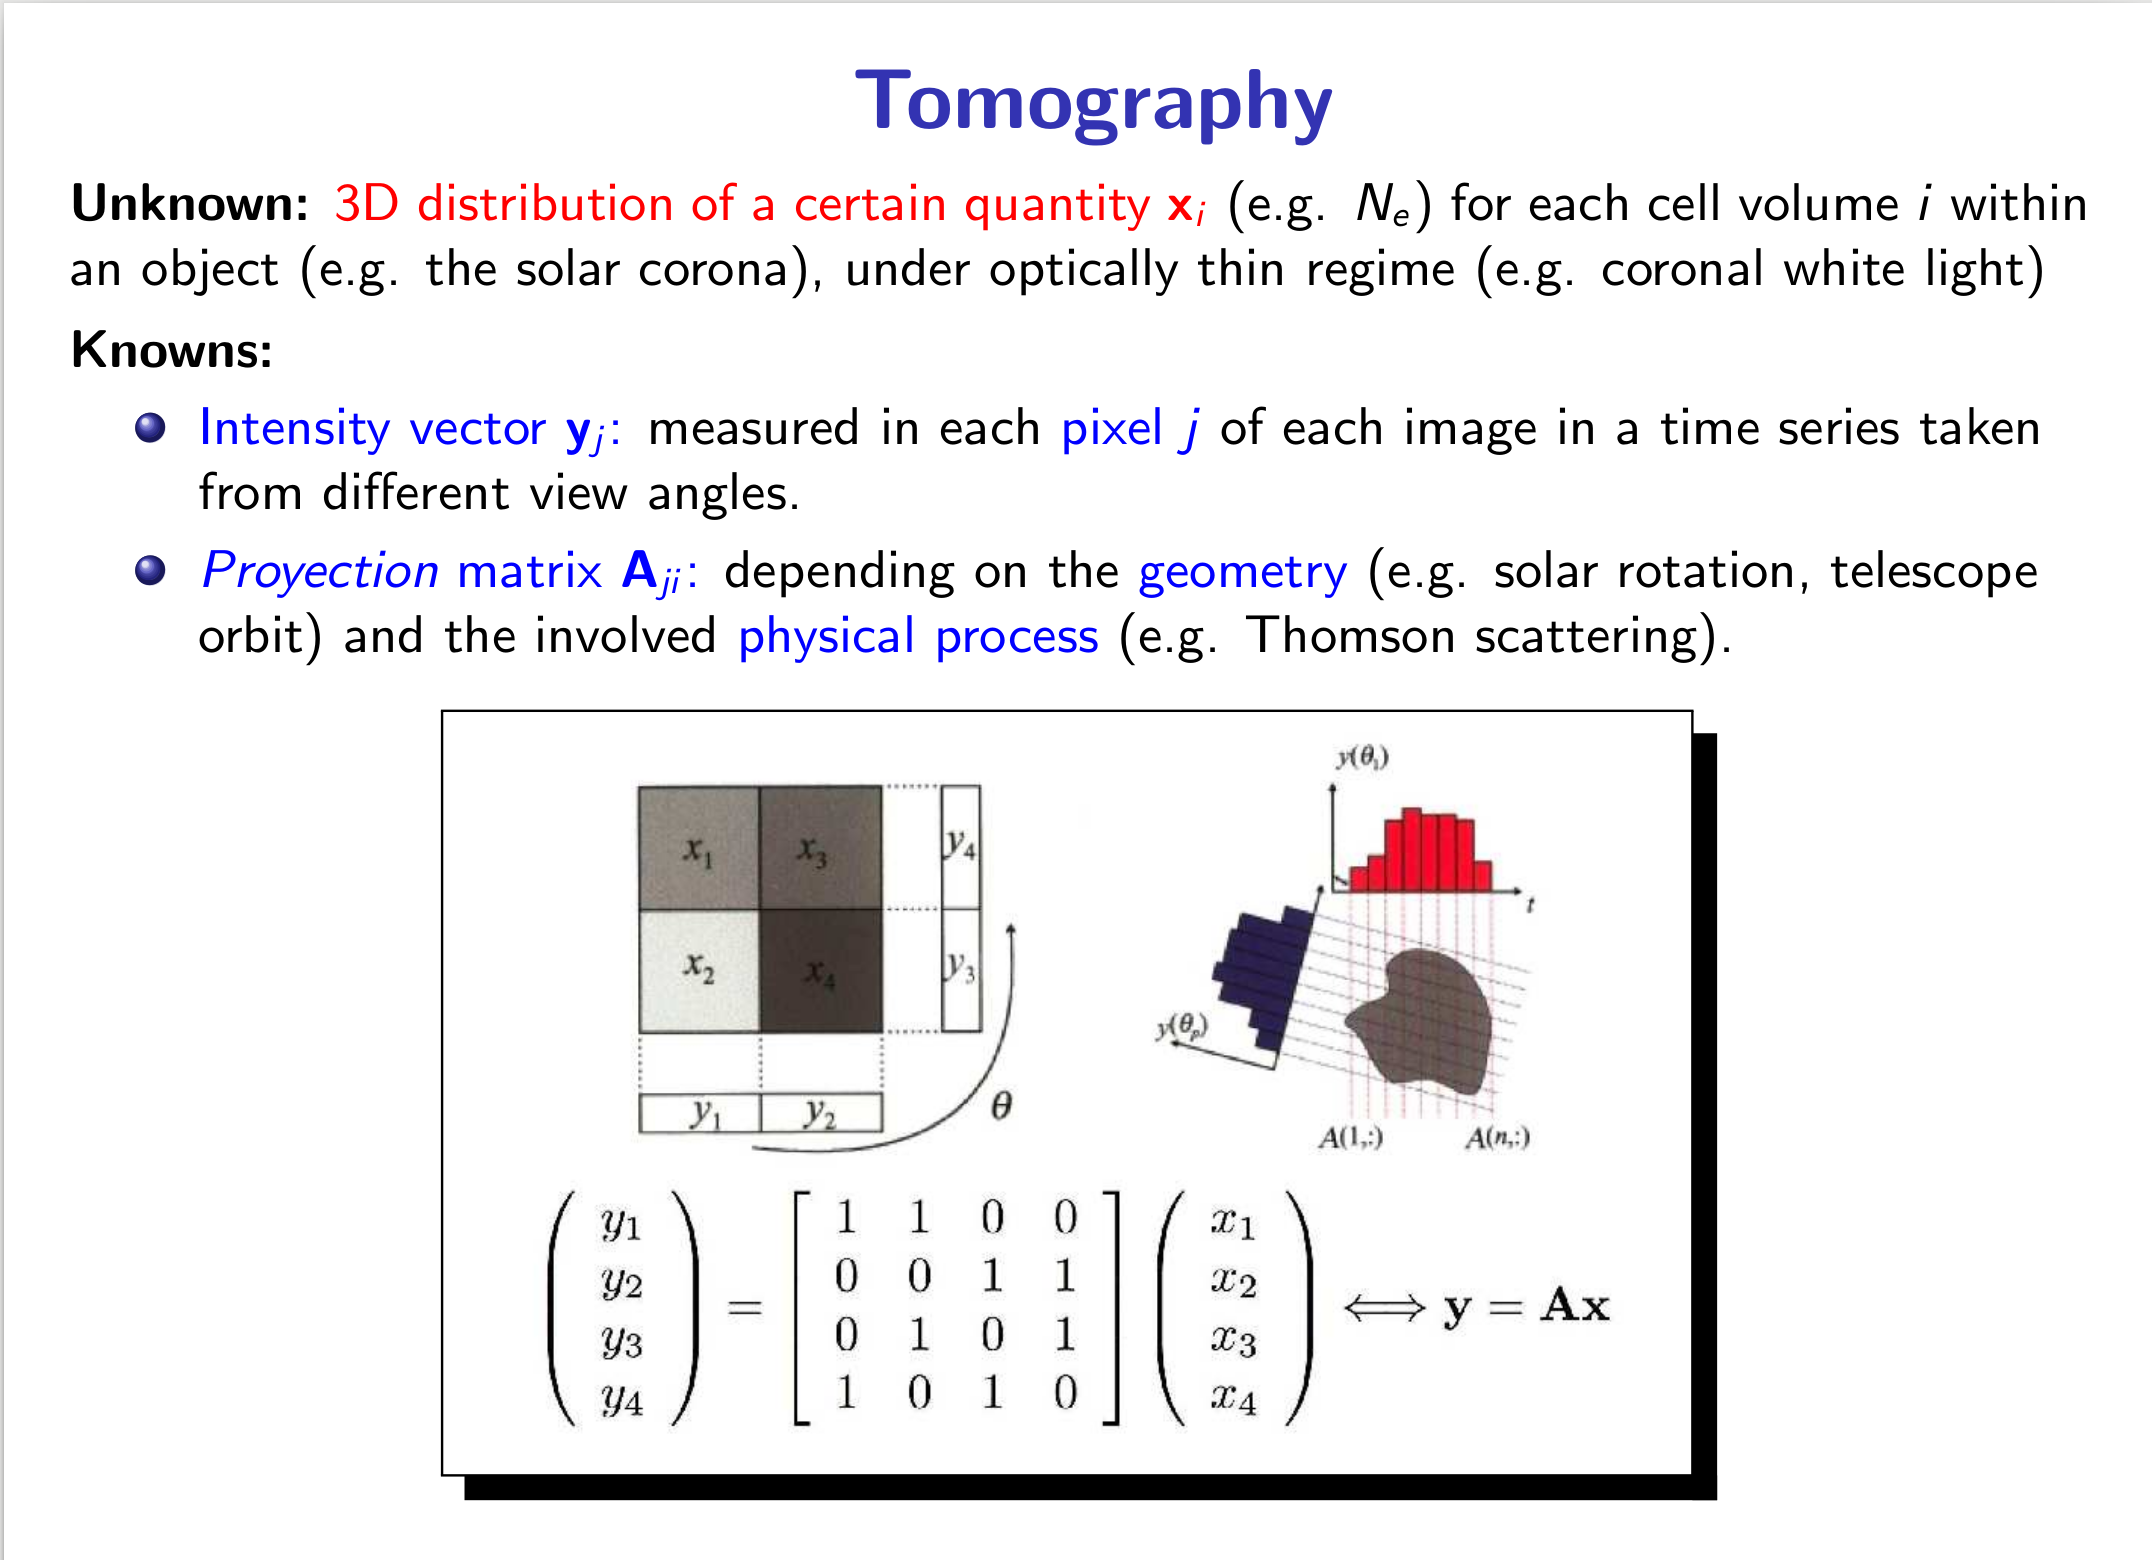
\includegraphics[width=0.33\textwidth]{tomo2.png}}
{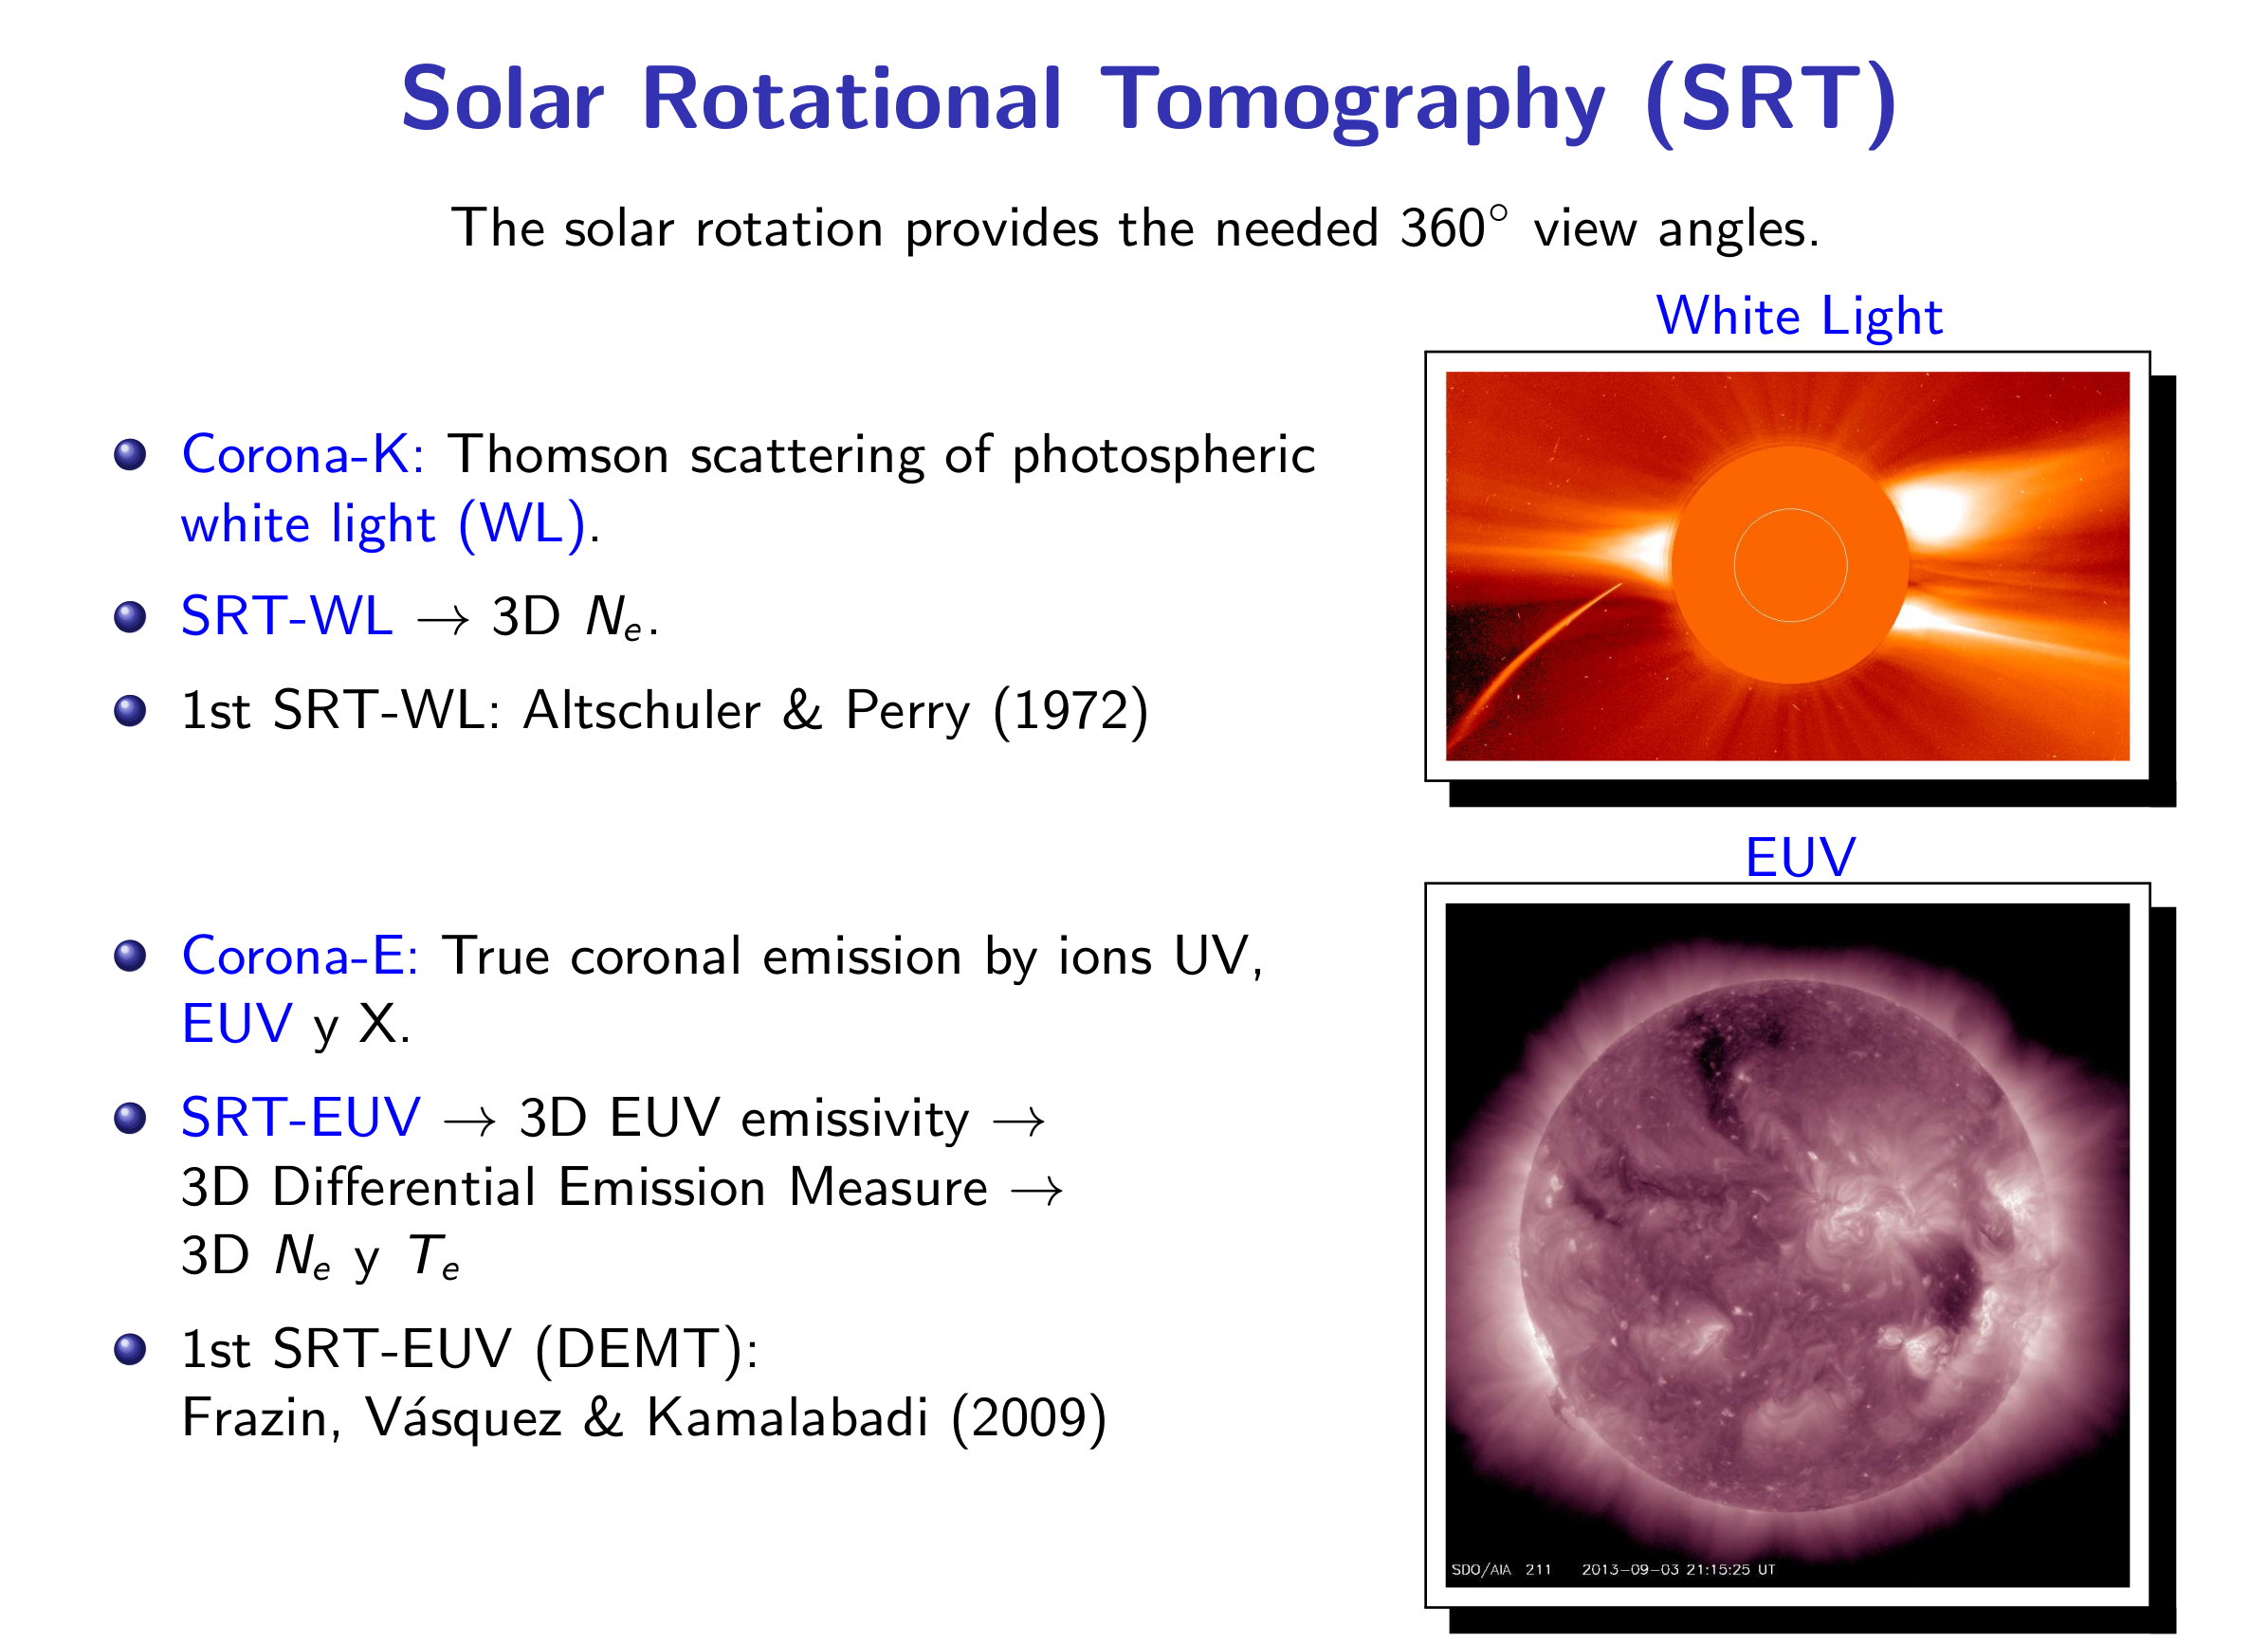
\includegraphics[width=0.33\textwidth]{tomo3.png}}
}
}

\headerbox{Data images}{name=Images,column=0,below=Tom,span=0.5}{
{\footnotesize\sf
\begin{center}
\azul{HAO/KCOR} white light\\
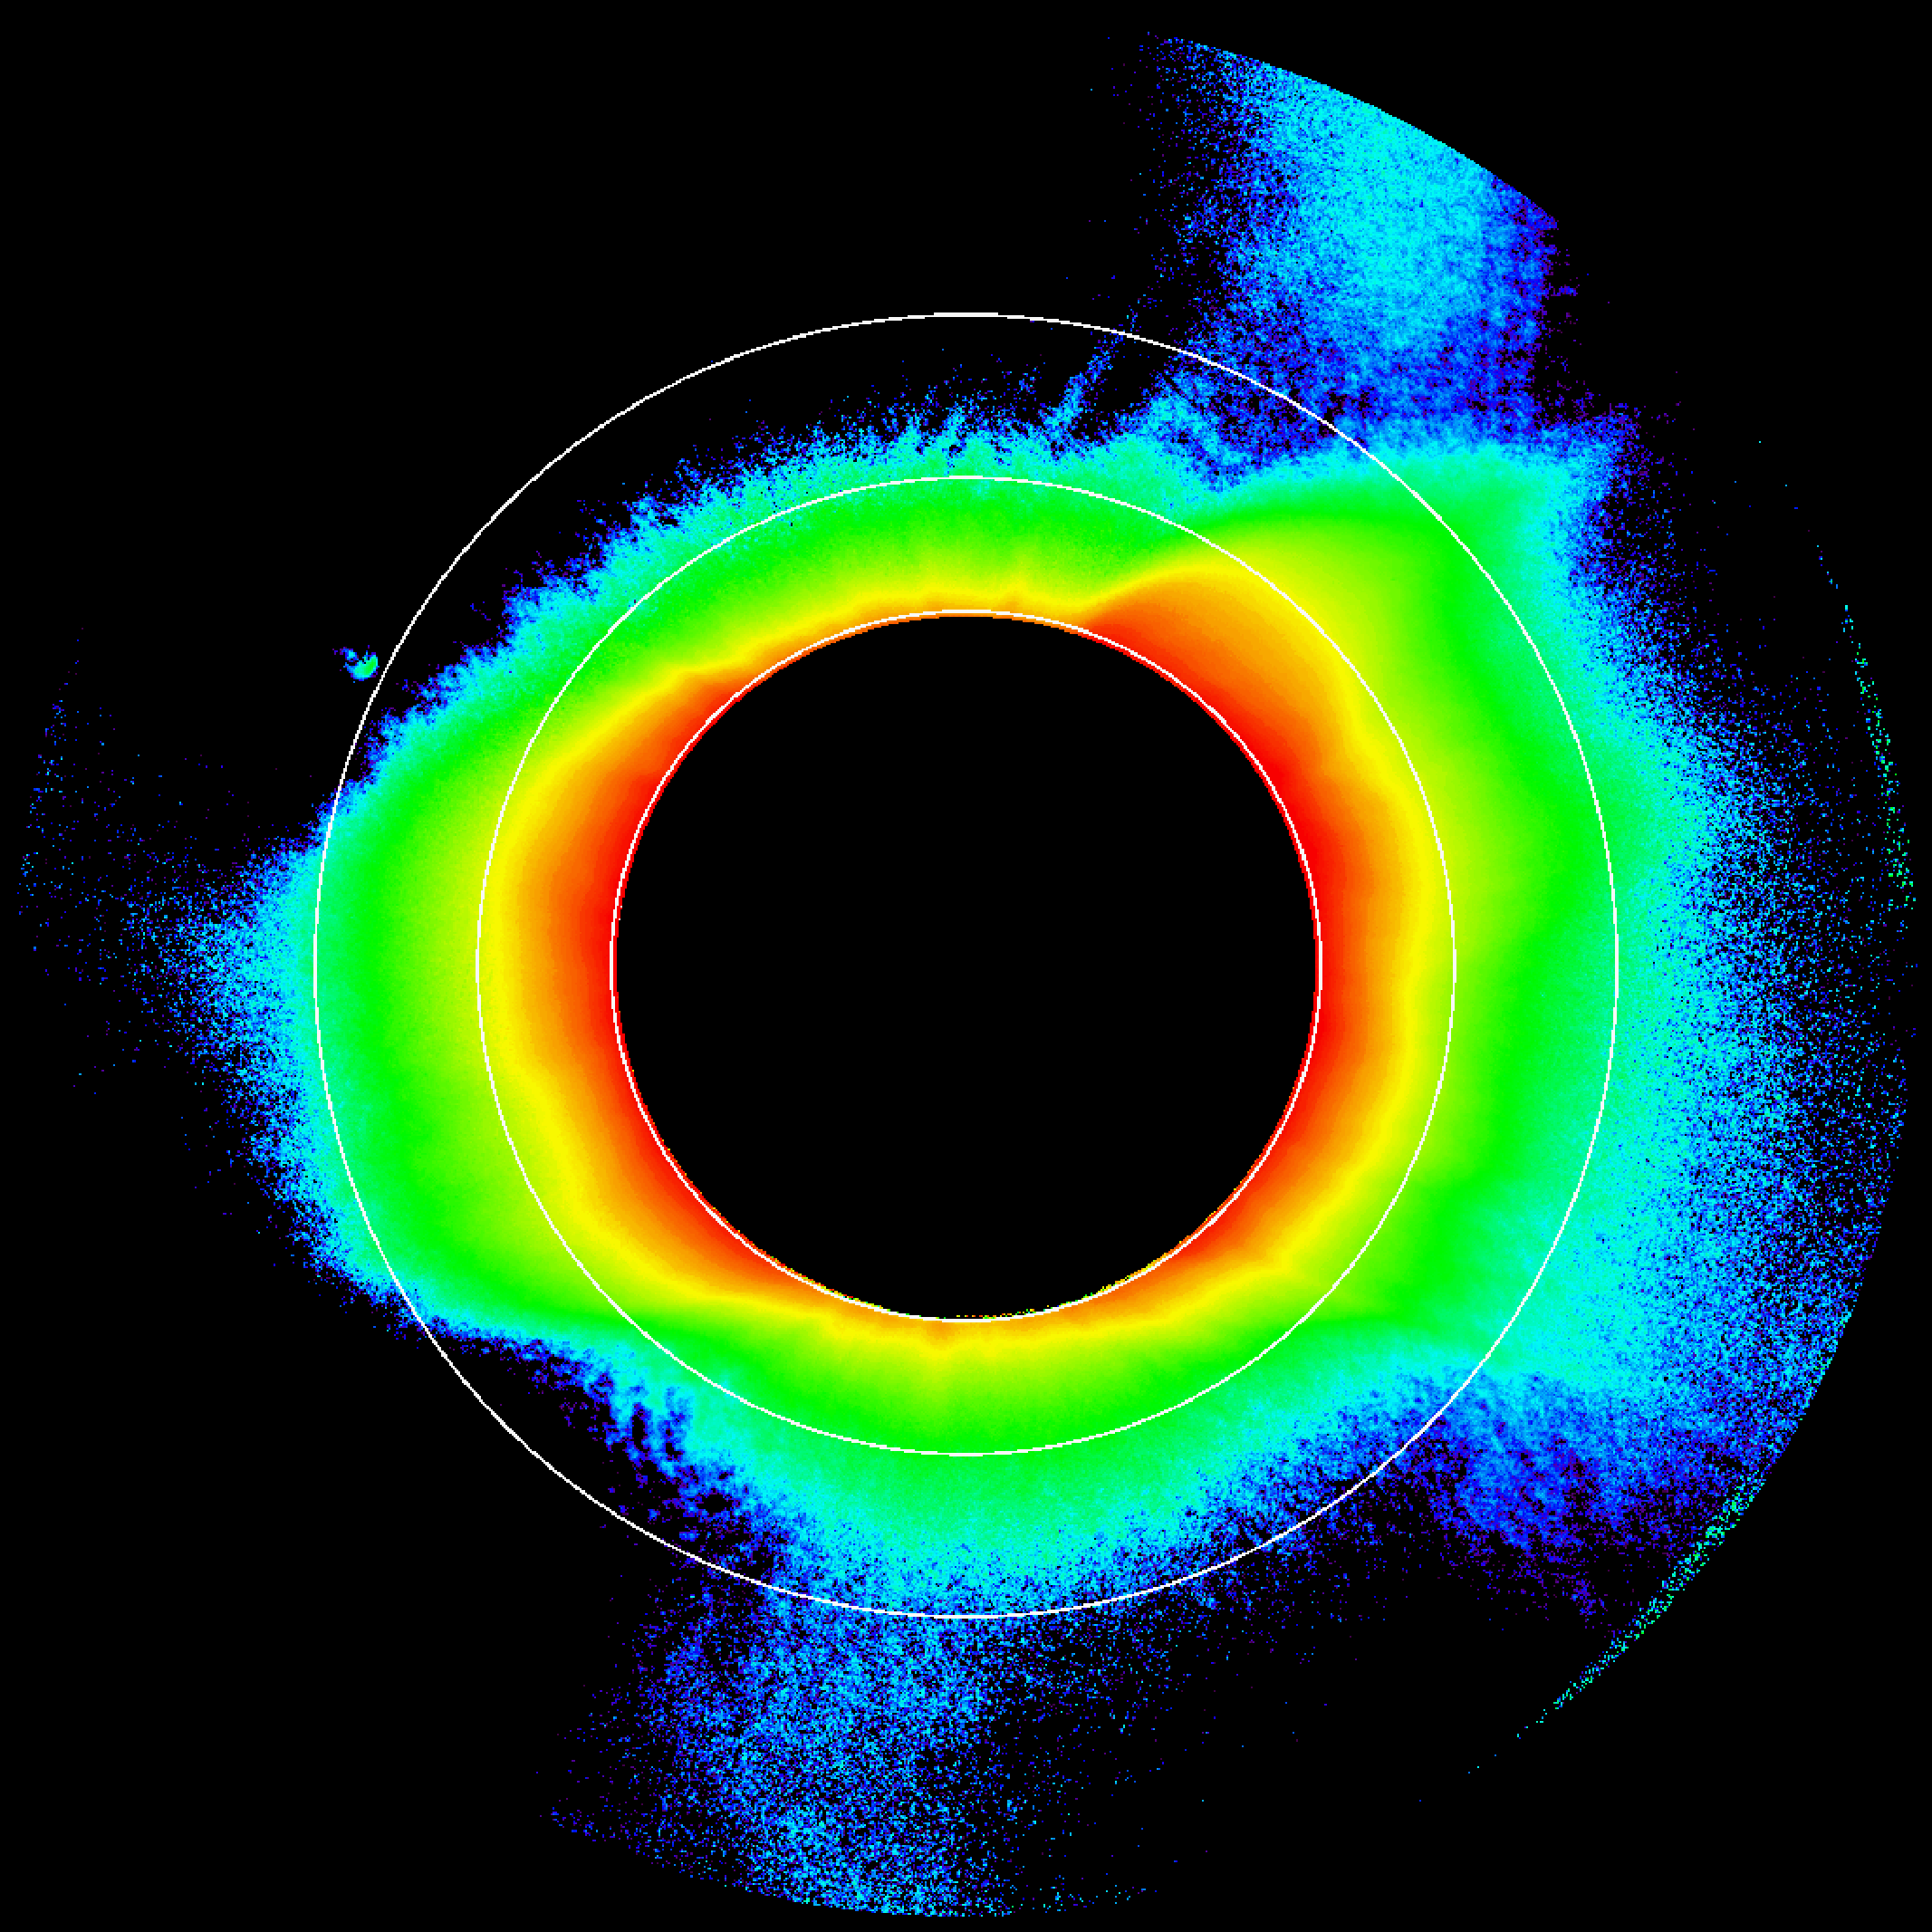
\includegraphics[width=0.9\columnwidth]{20171203_180316_kcor_l1_10min_avg_image.pdf}\\
\azul{SDO/AIA-171\,\AA} band\\
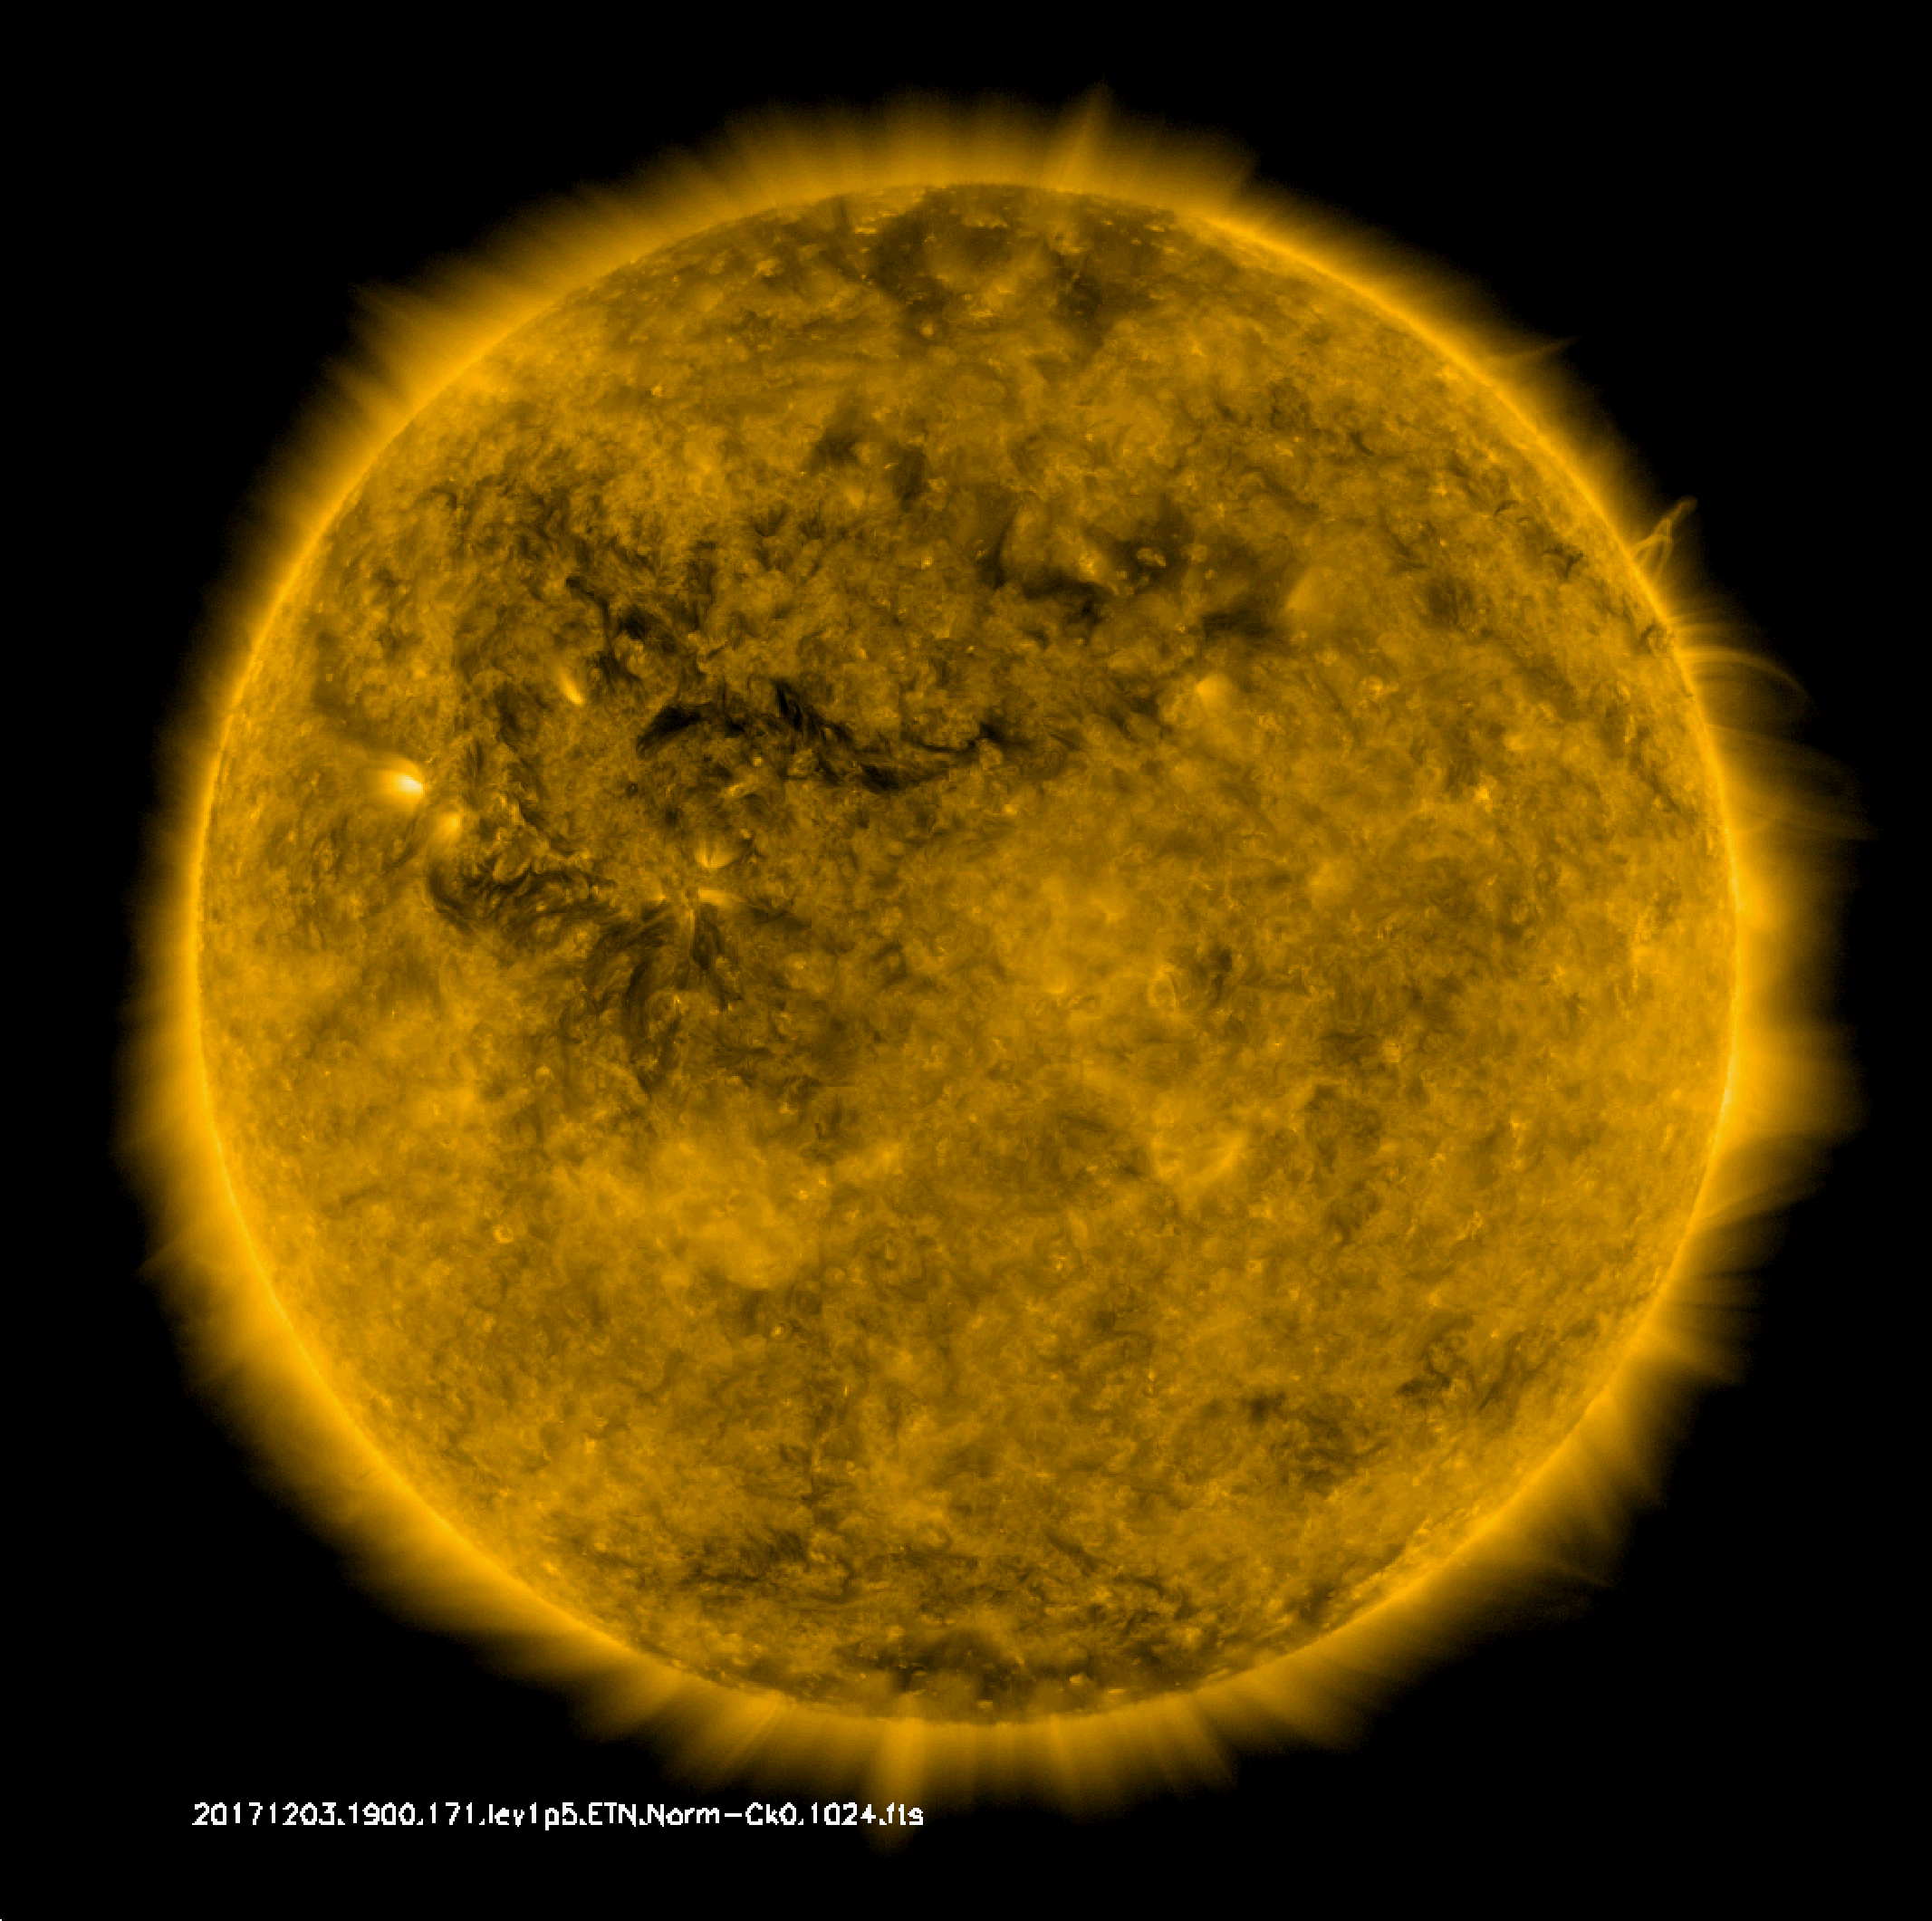
\includegraphics[width=0.9\columnwidth]{img_171.pdf}\\
\azul{SDO/AIA-193\,\AA} band\\
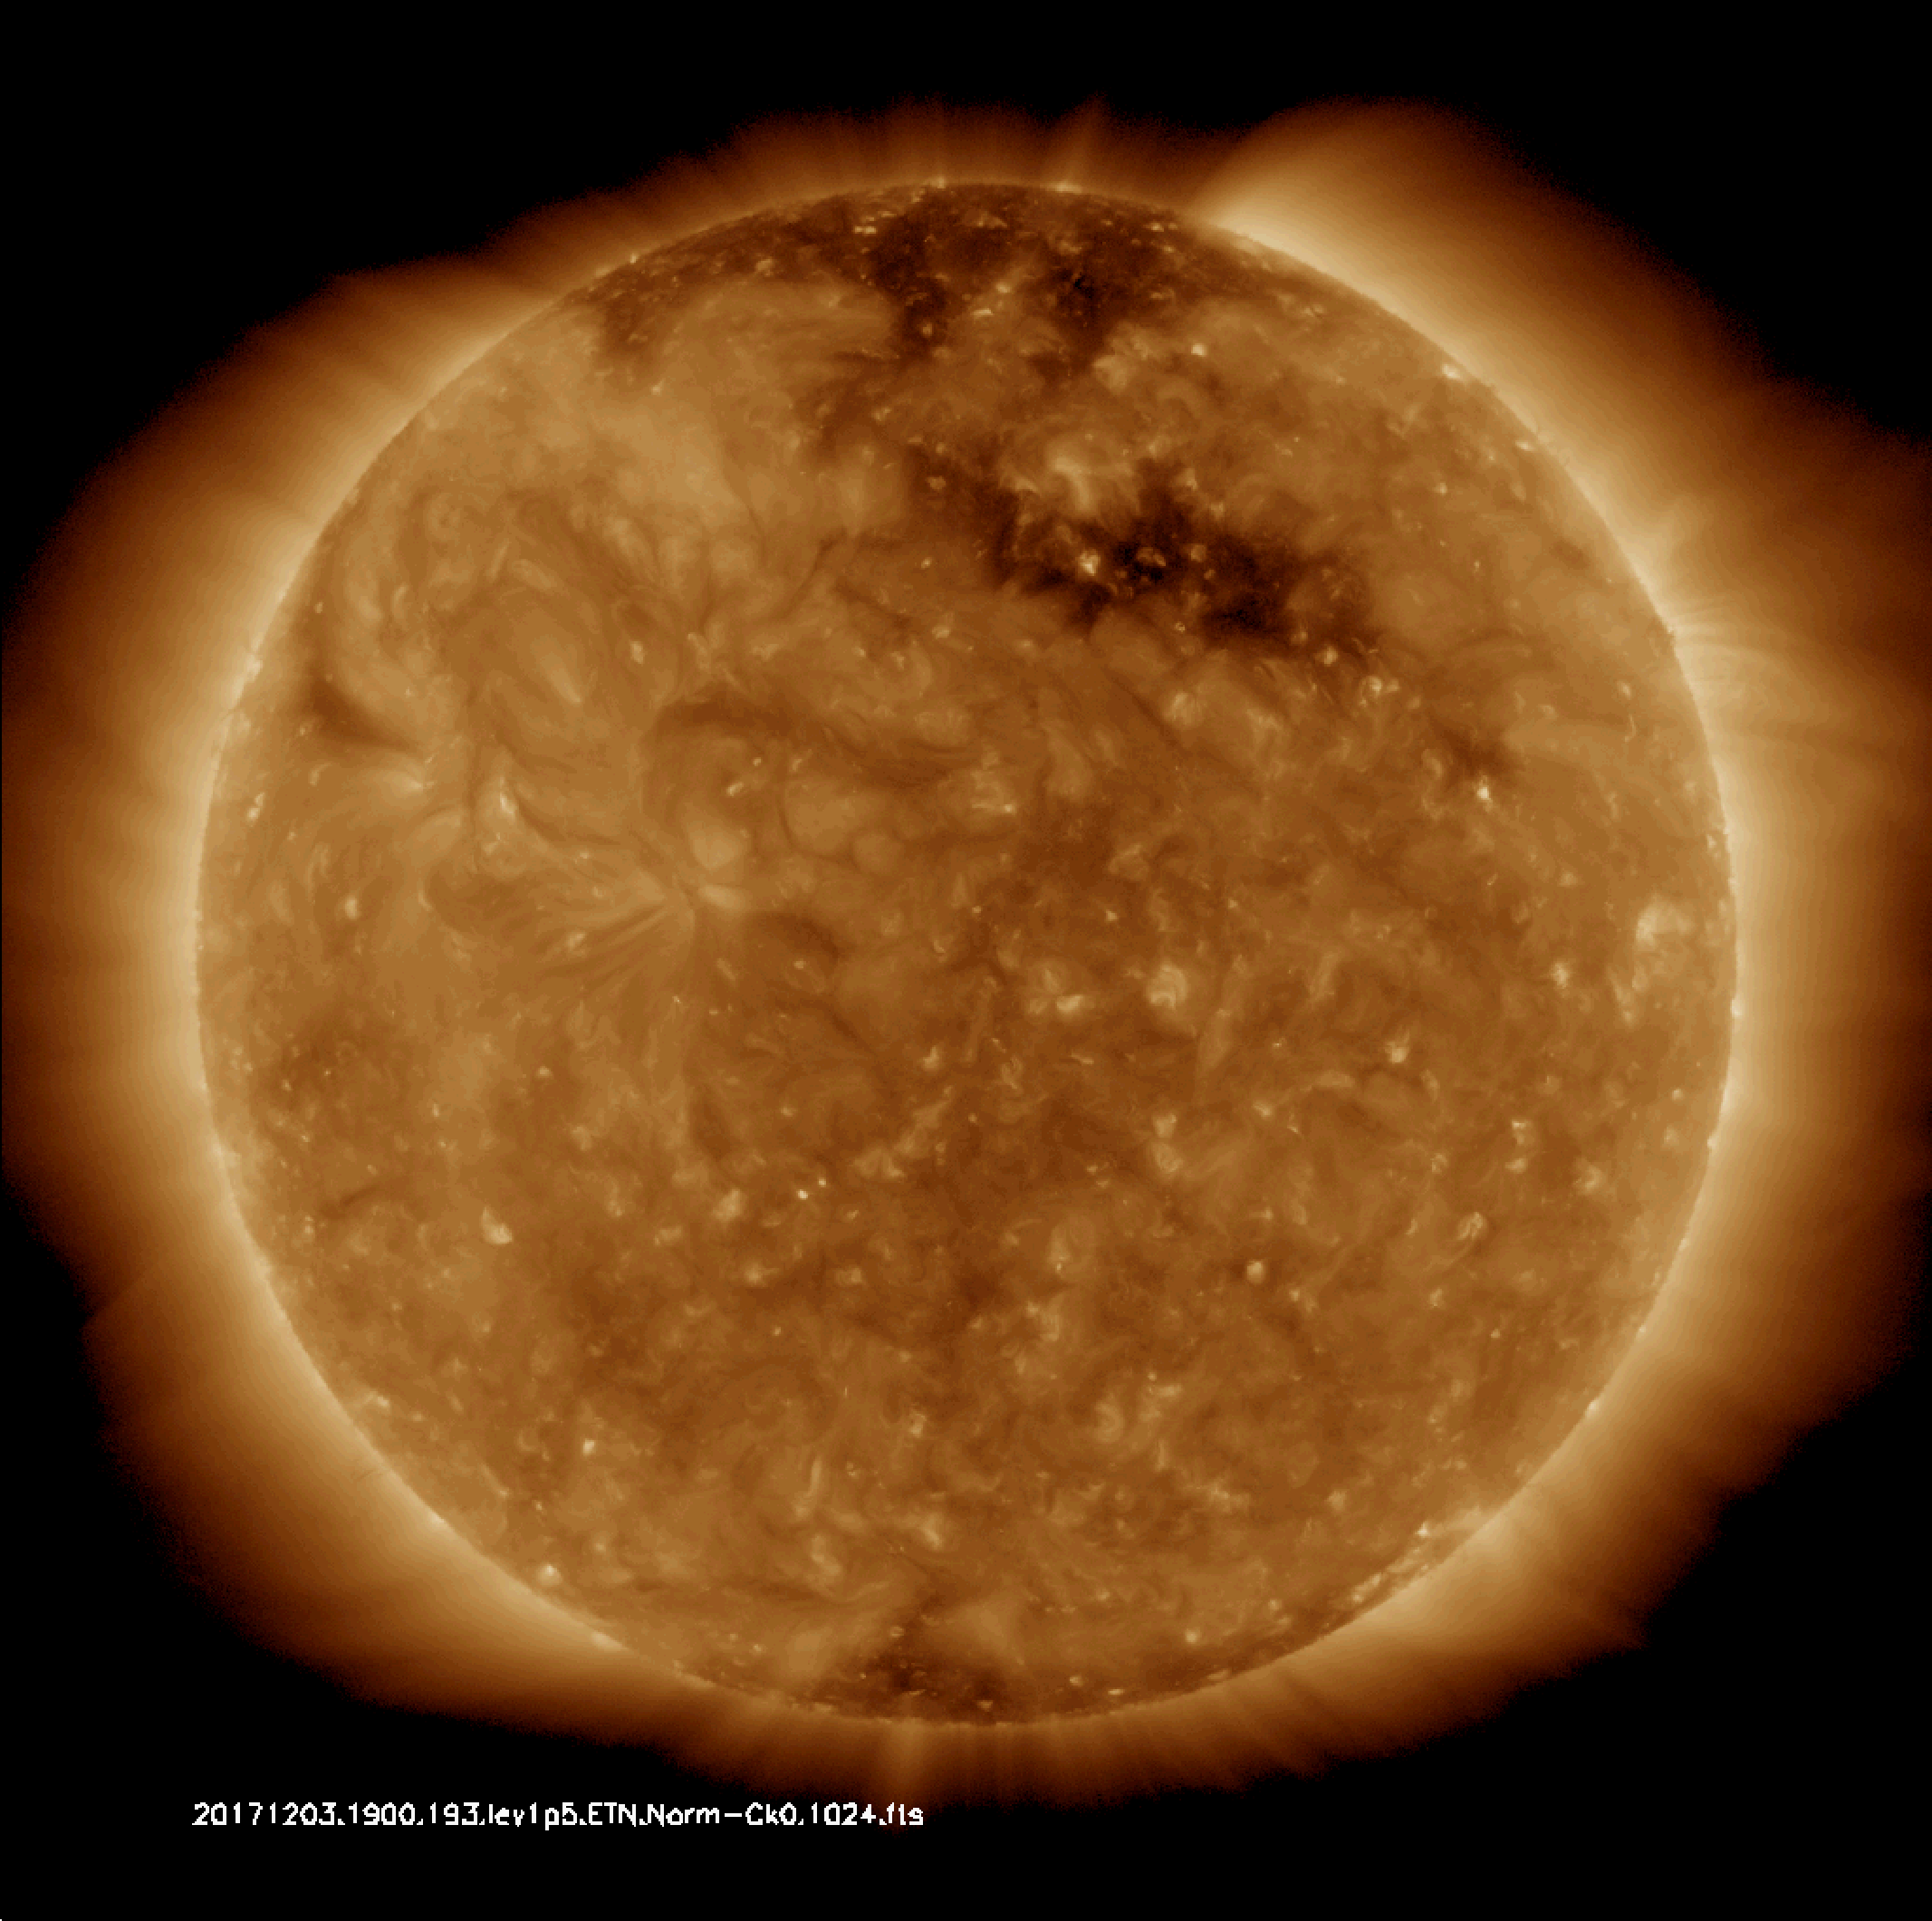
\includegraphics[width=0.9\columnwidth]{img_193.pdf}\\
\azul{SDO/AIA-211\,\AA} band\\
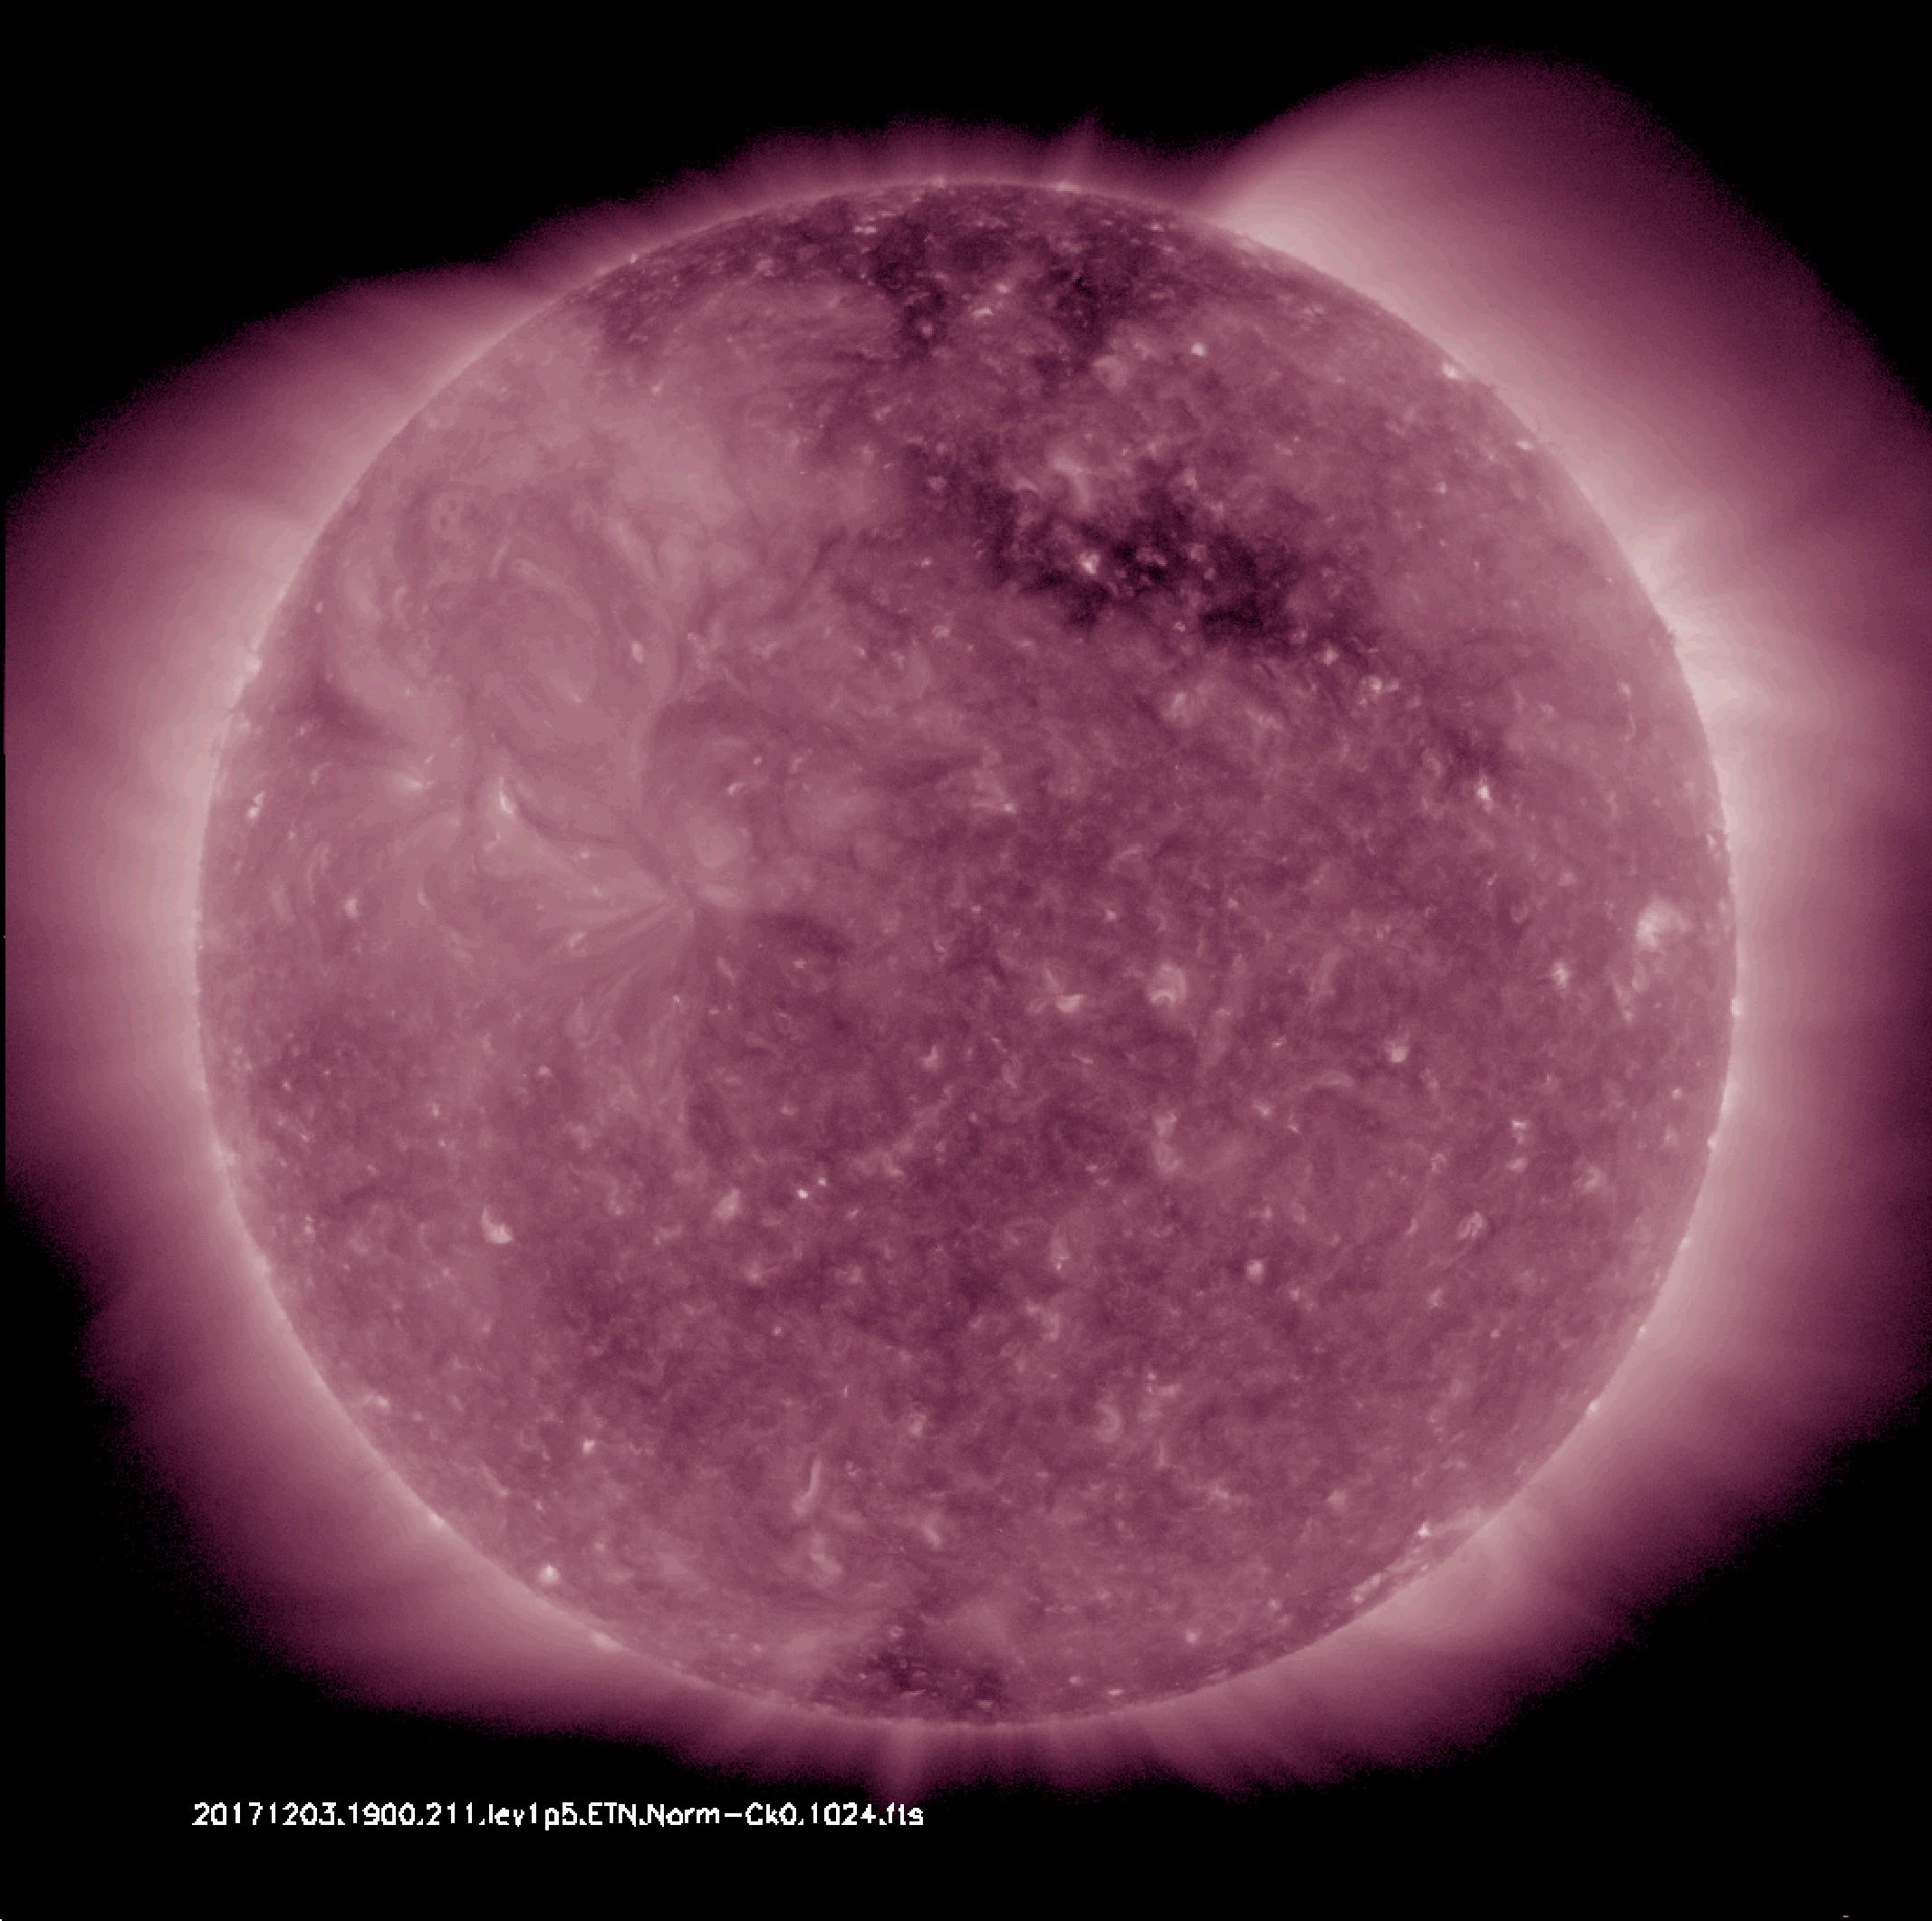
\includegraphics[width=0.9\columnwidth]{img_211.pdf}\\
\azul{HAO/CoMP-1074\,\AA} line\\
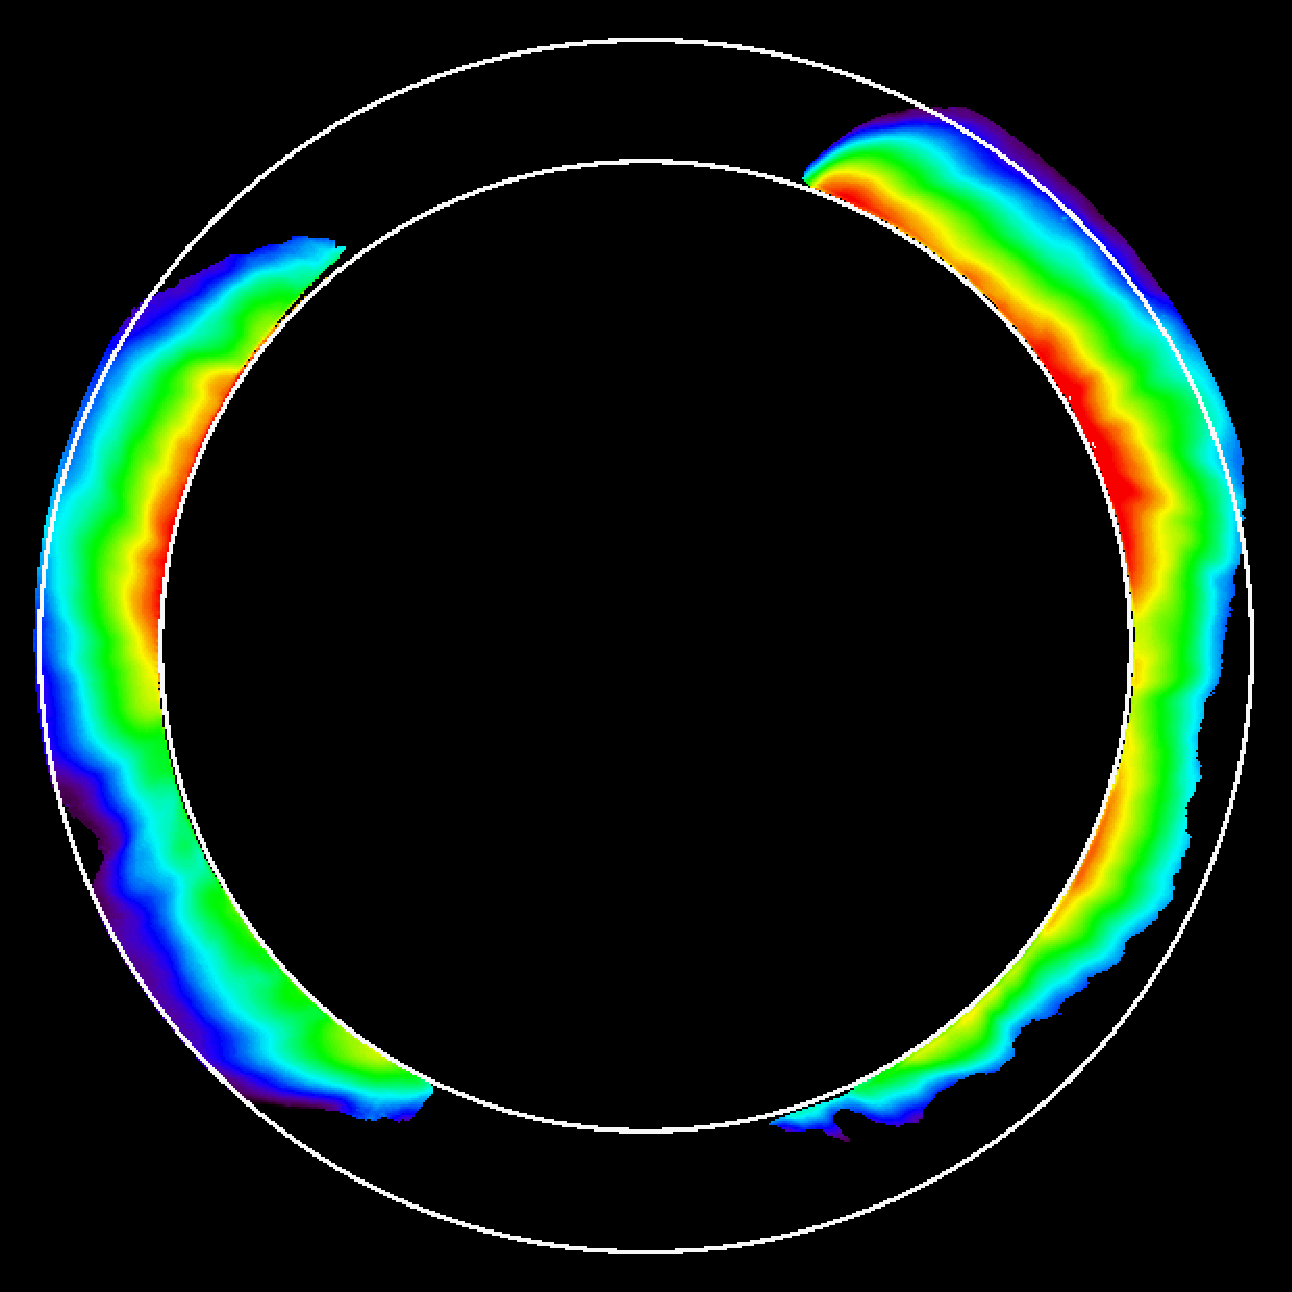
\includegraphics[width=0.9\columnwidth]{20171203_214113_comp_1074_dynamics_avg_total_intensity_t018-Dt8_images.pdf}\\
\azul{HAO/CoMP-1079\,\AA} line\\
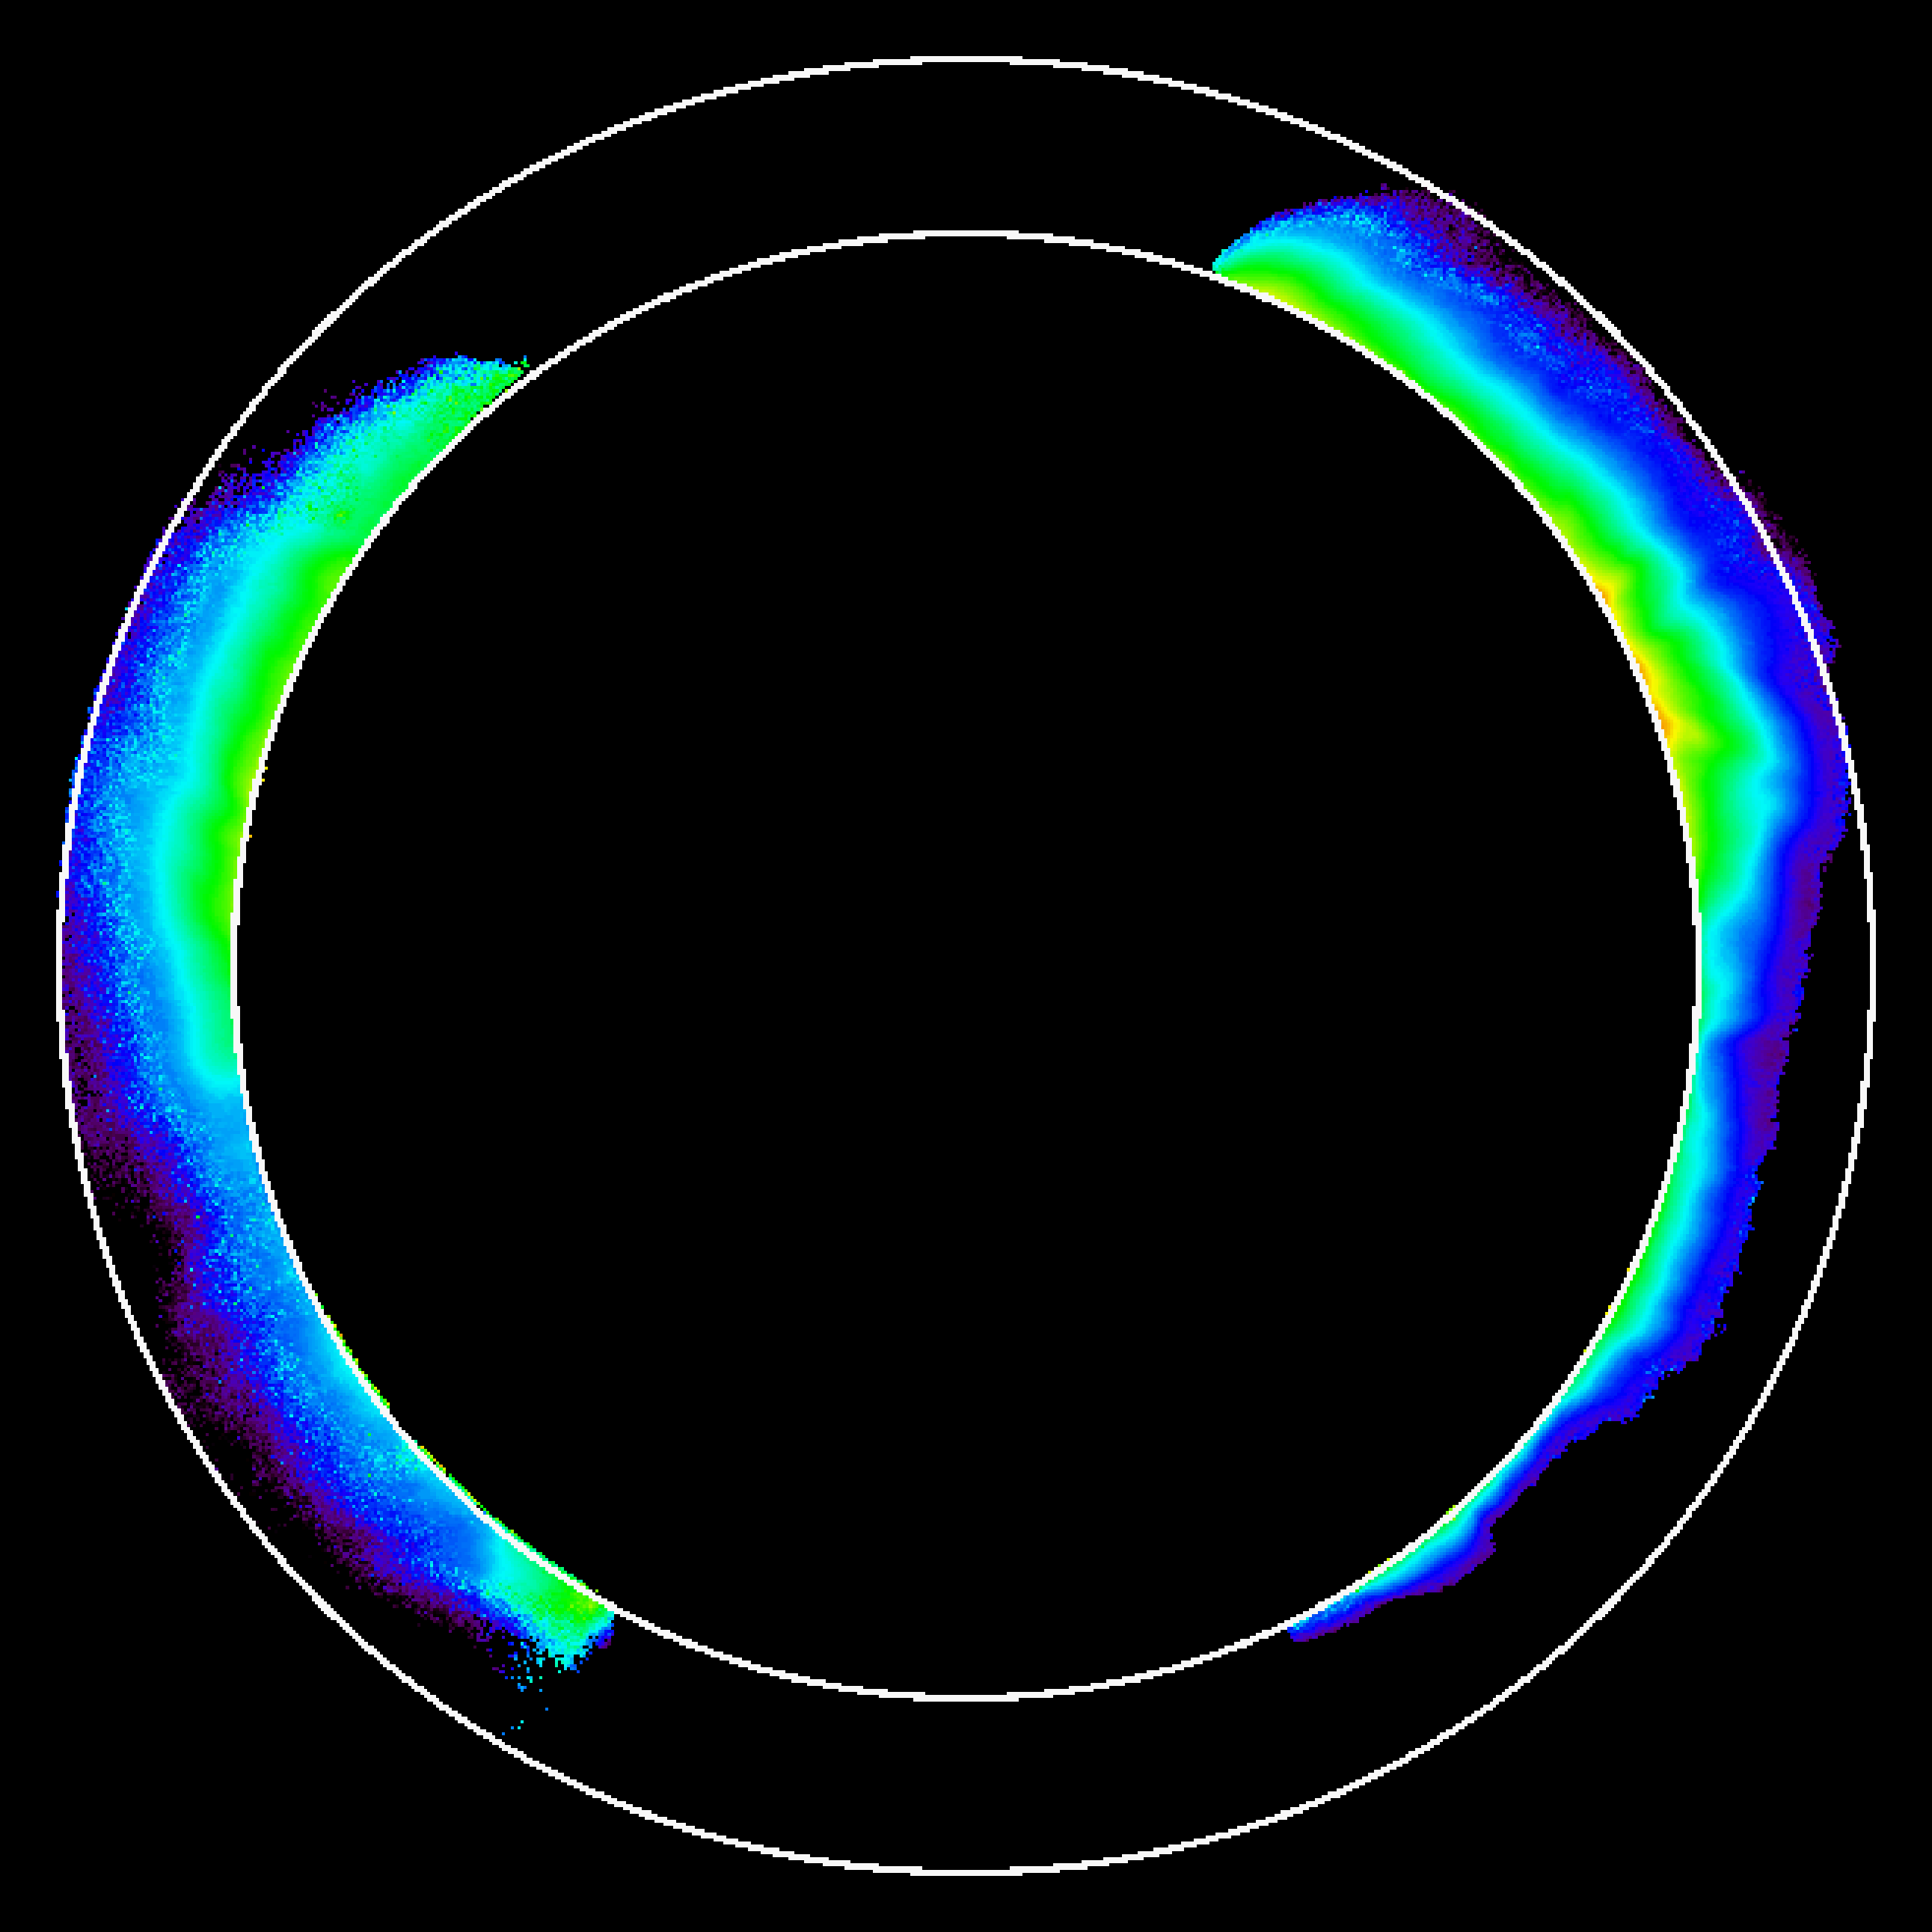
\includegraphics[width=0.9\columnwidth]{20171203_202649_comp_1079_dynamics_avg_total_intensity_t018-Dt8.pdf}
\vskip 0.1cm
\azul{Common FOV: $\approx 1.05-1.25\,\mrsun$}
\end{center}
}
}

\headerbox{Tomographic Reconstructions}{name=Reconstructions,column=0.5,below=Tom,span=0.9}{
{\footnotesize\sf
\begin{center}
Carrington maps at a sample height\\
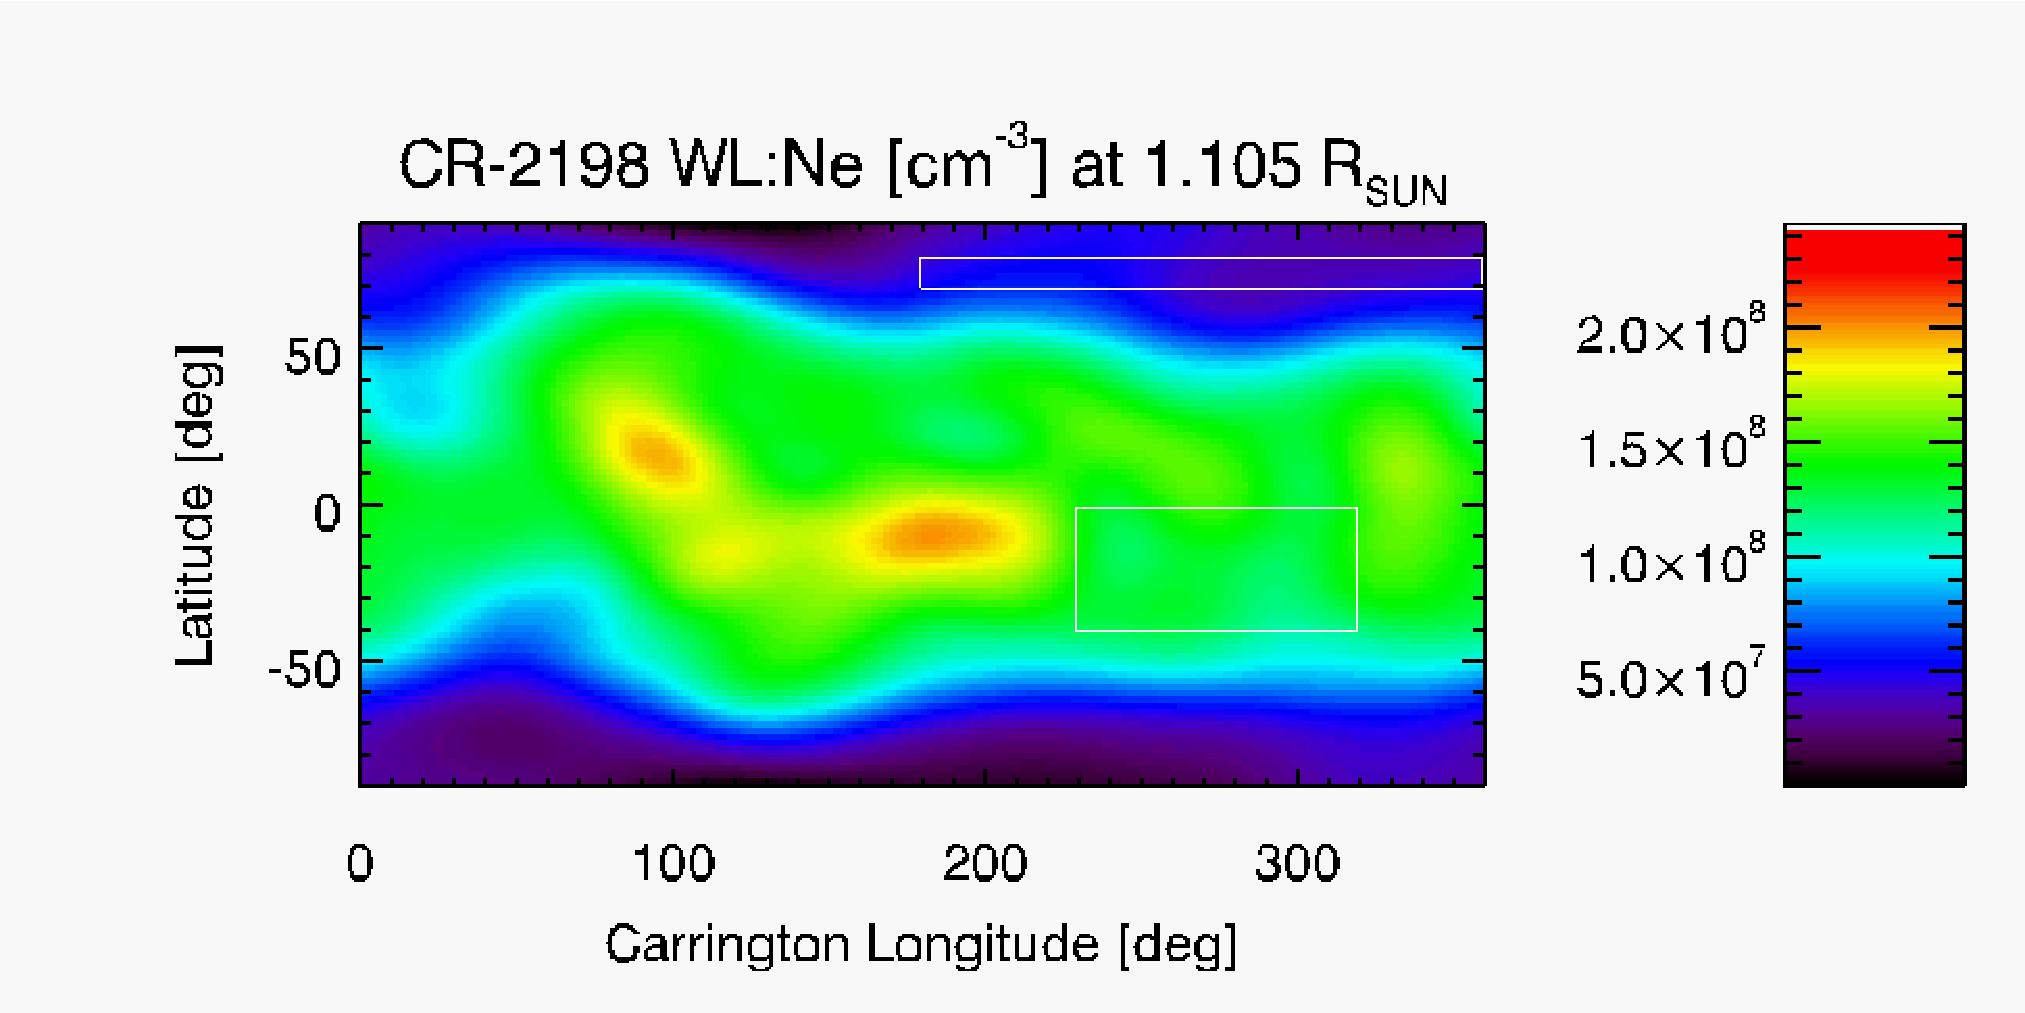
\includegraphics[width=\columnwidth]{map_x_KCORCR219813imgs-reducedbf2ri105ro225_Inst_109_200_120_90_180_dropneg_r3D_l1e-4_1105_Rsun.pdf}\\
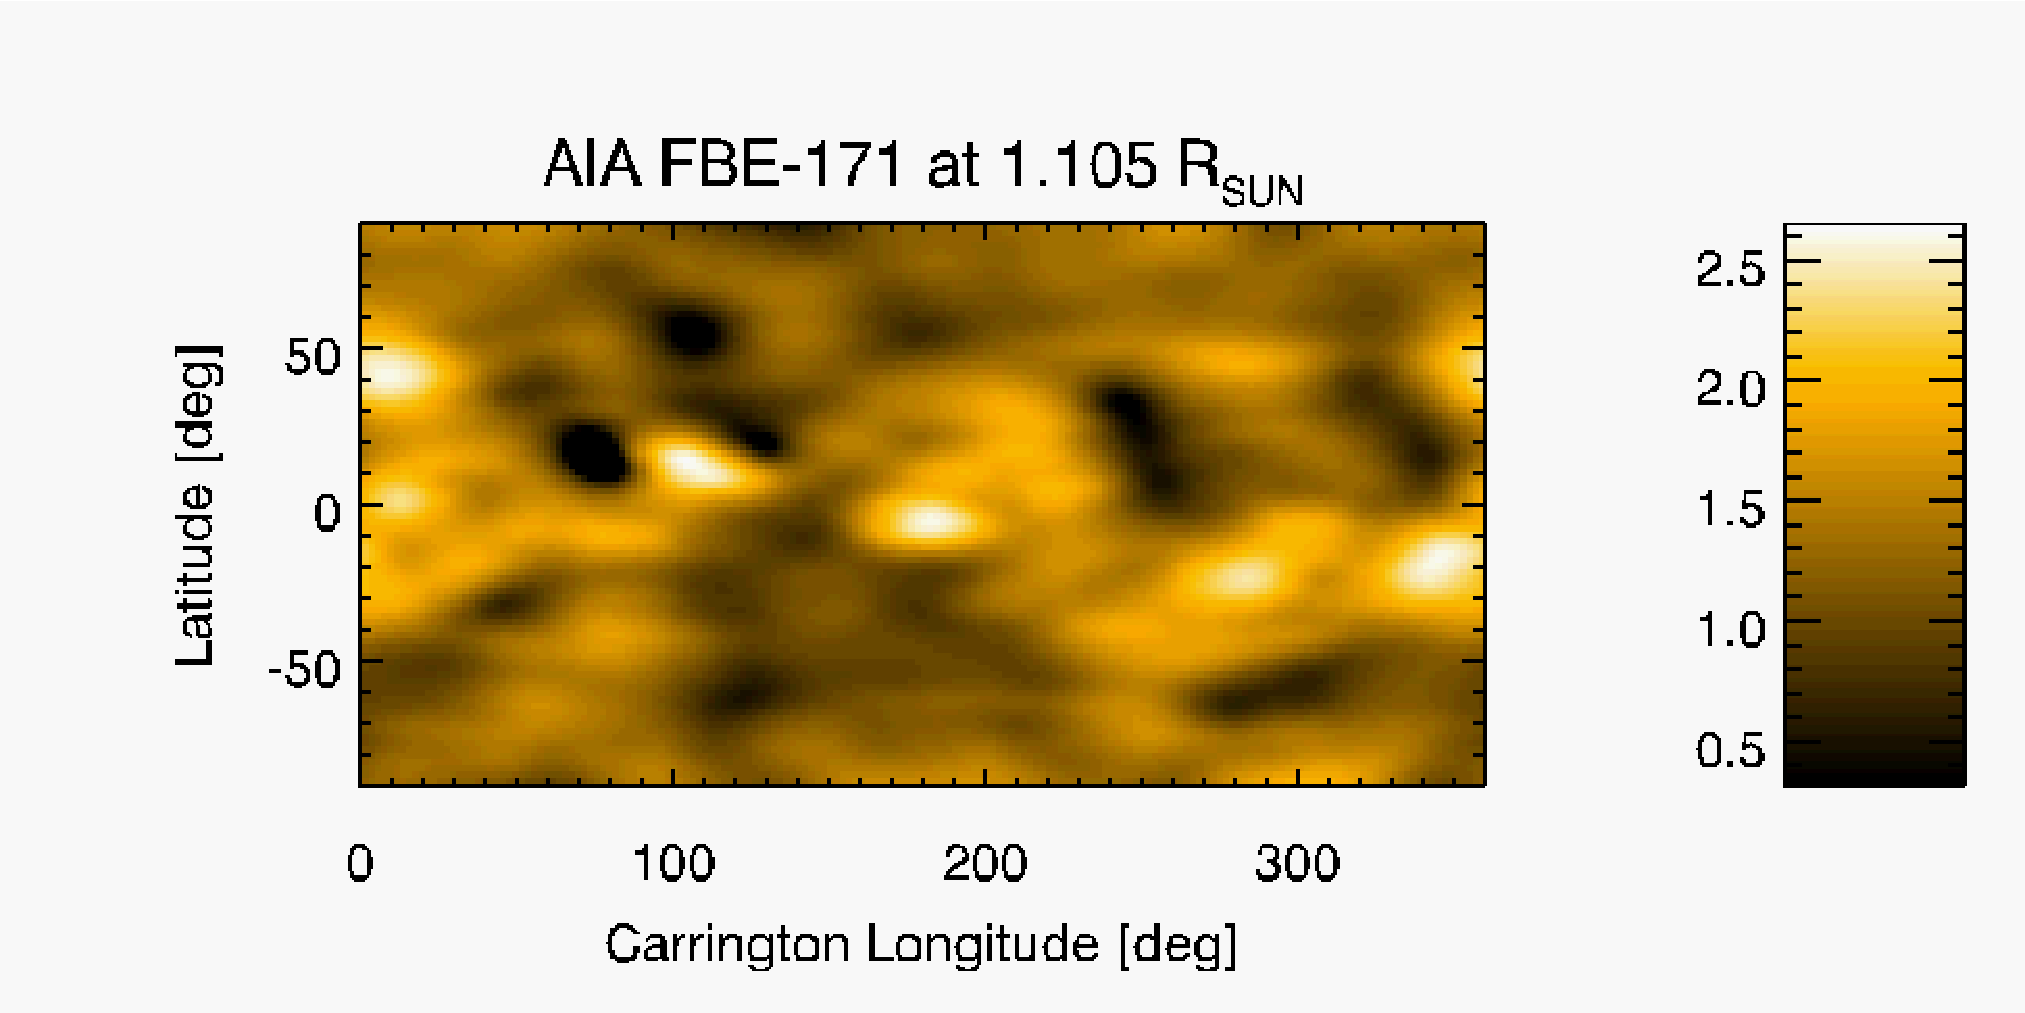
\includegraphics[width=\columnwidth]{map_x_aia_171_1105_Rsun.pdf}\\
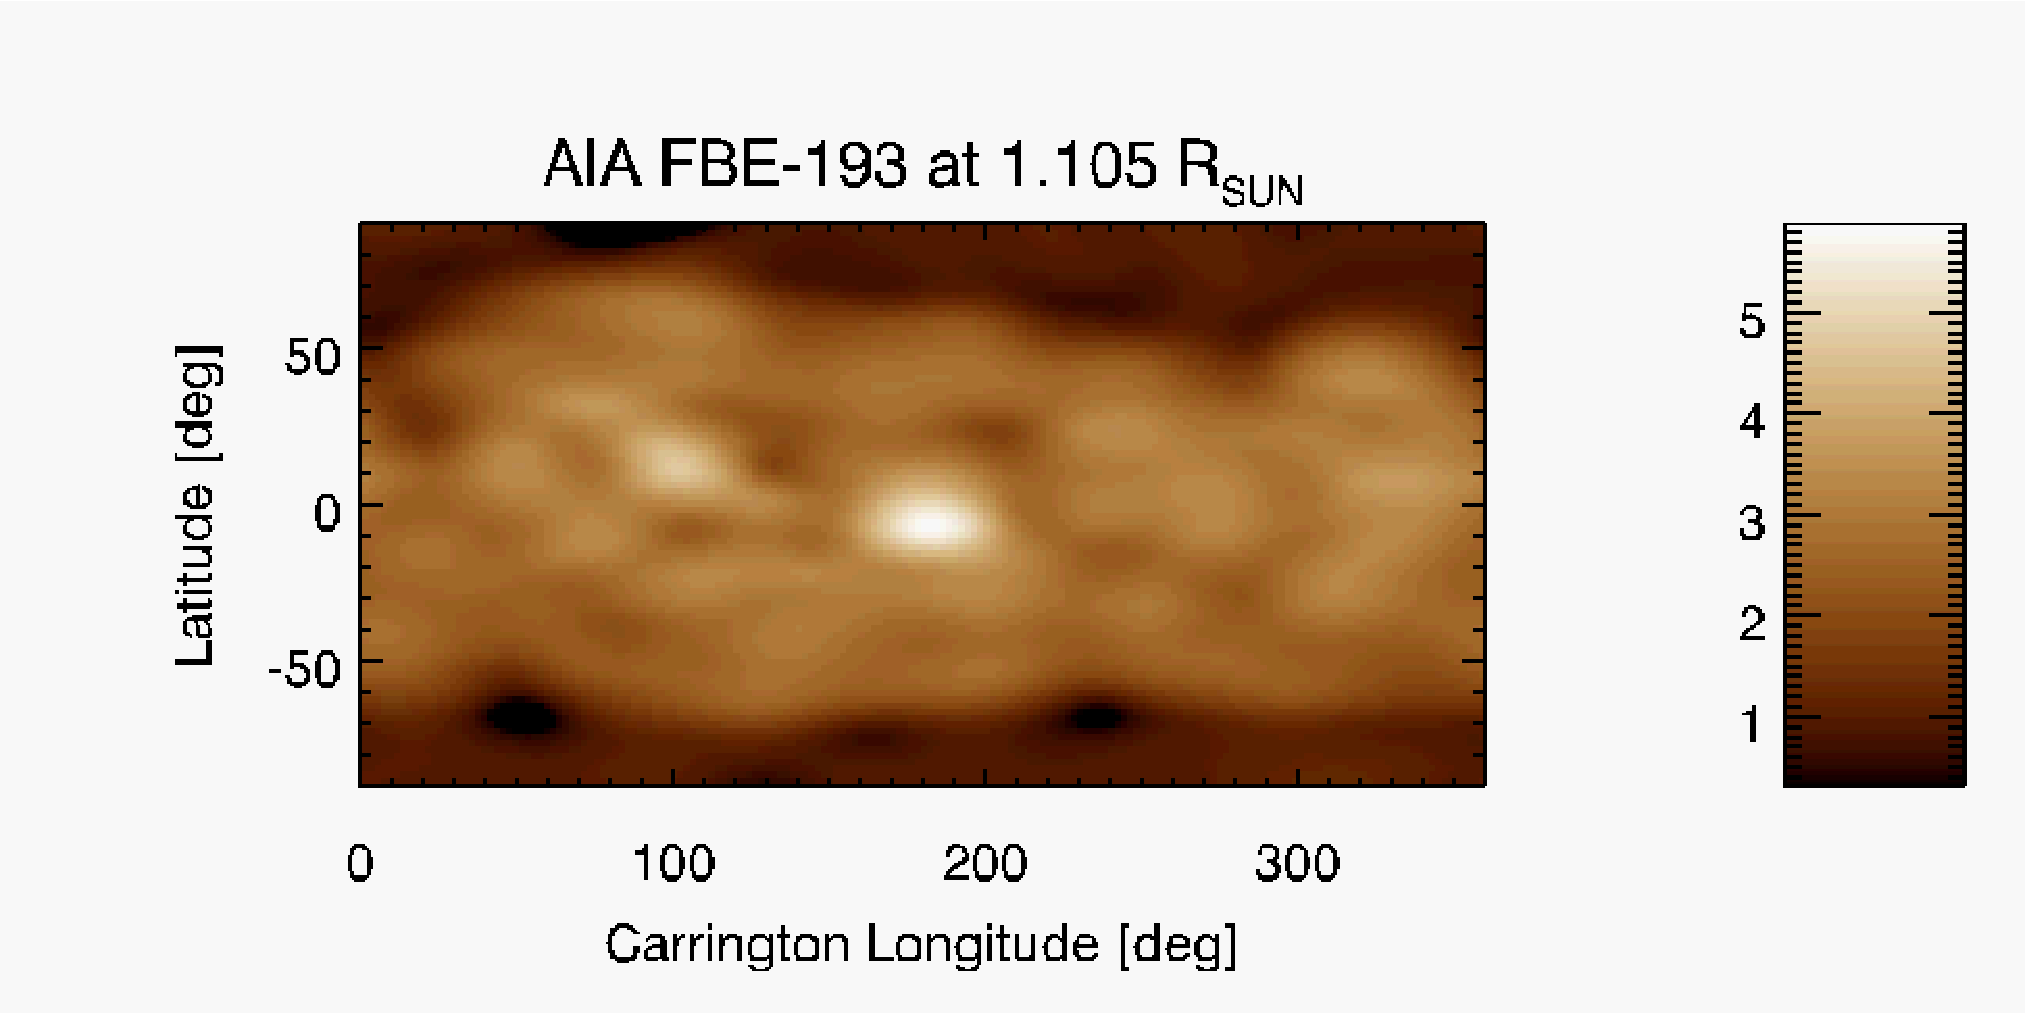
\includegraphics[width=\columnwidth]{map_x_aia_193_1105_Rsun.pdf}\\
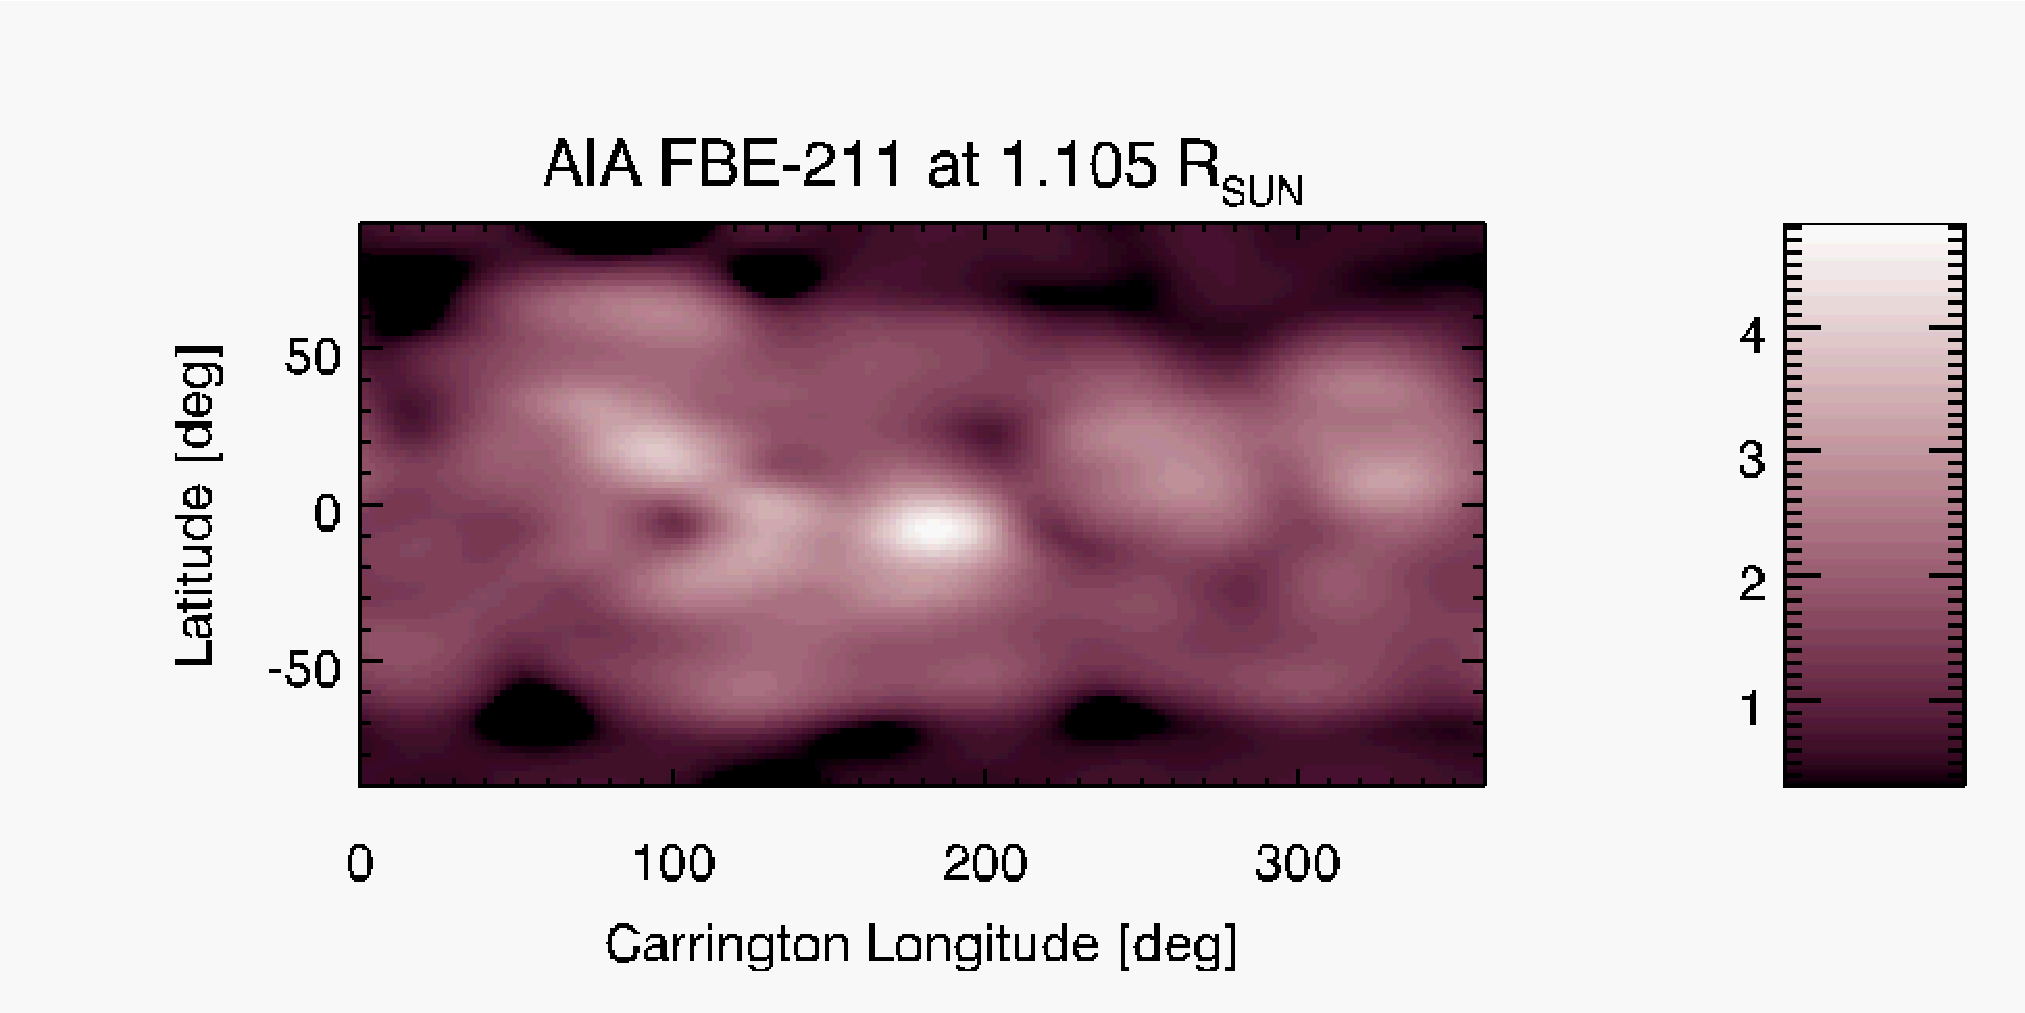
\includegraphics[width=\columnwidth]{map_x_aia_211_1105_Rsun.pdf}\\
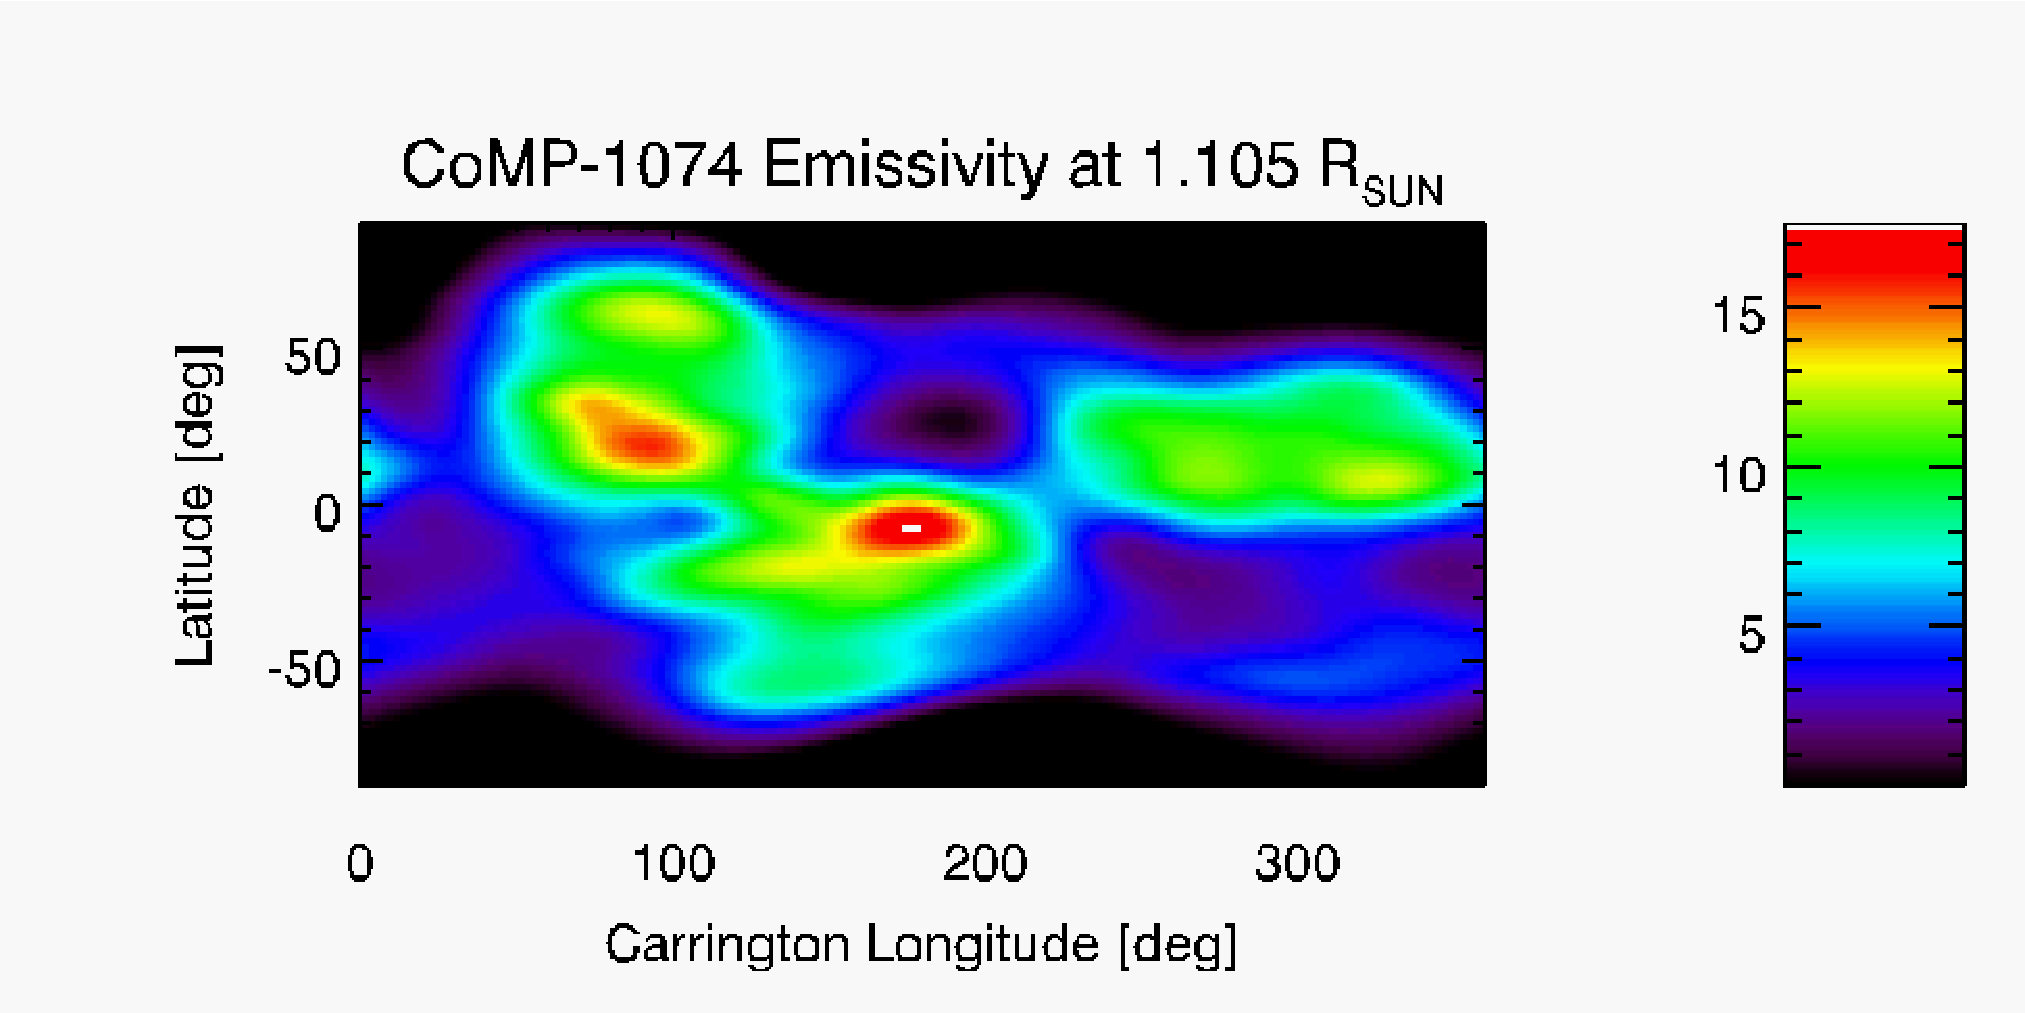
\includegraphics[width=\columnwidth]{map_x_comp1074_1105_Rsun.pdf}\\
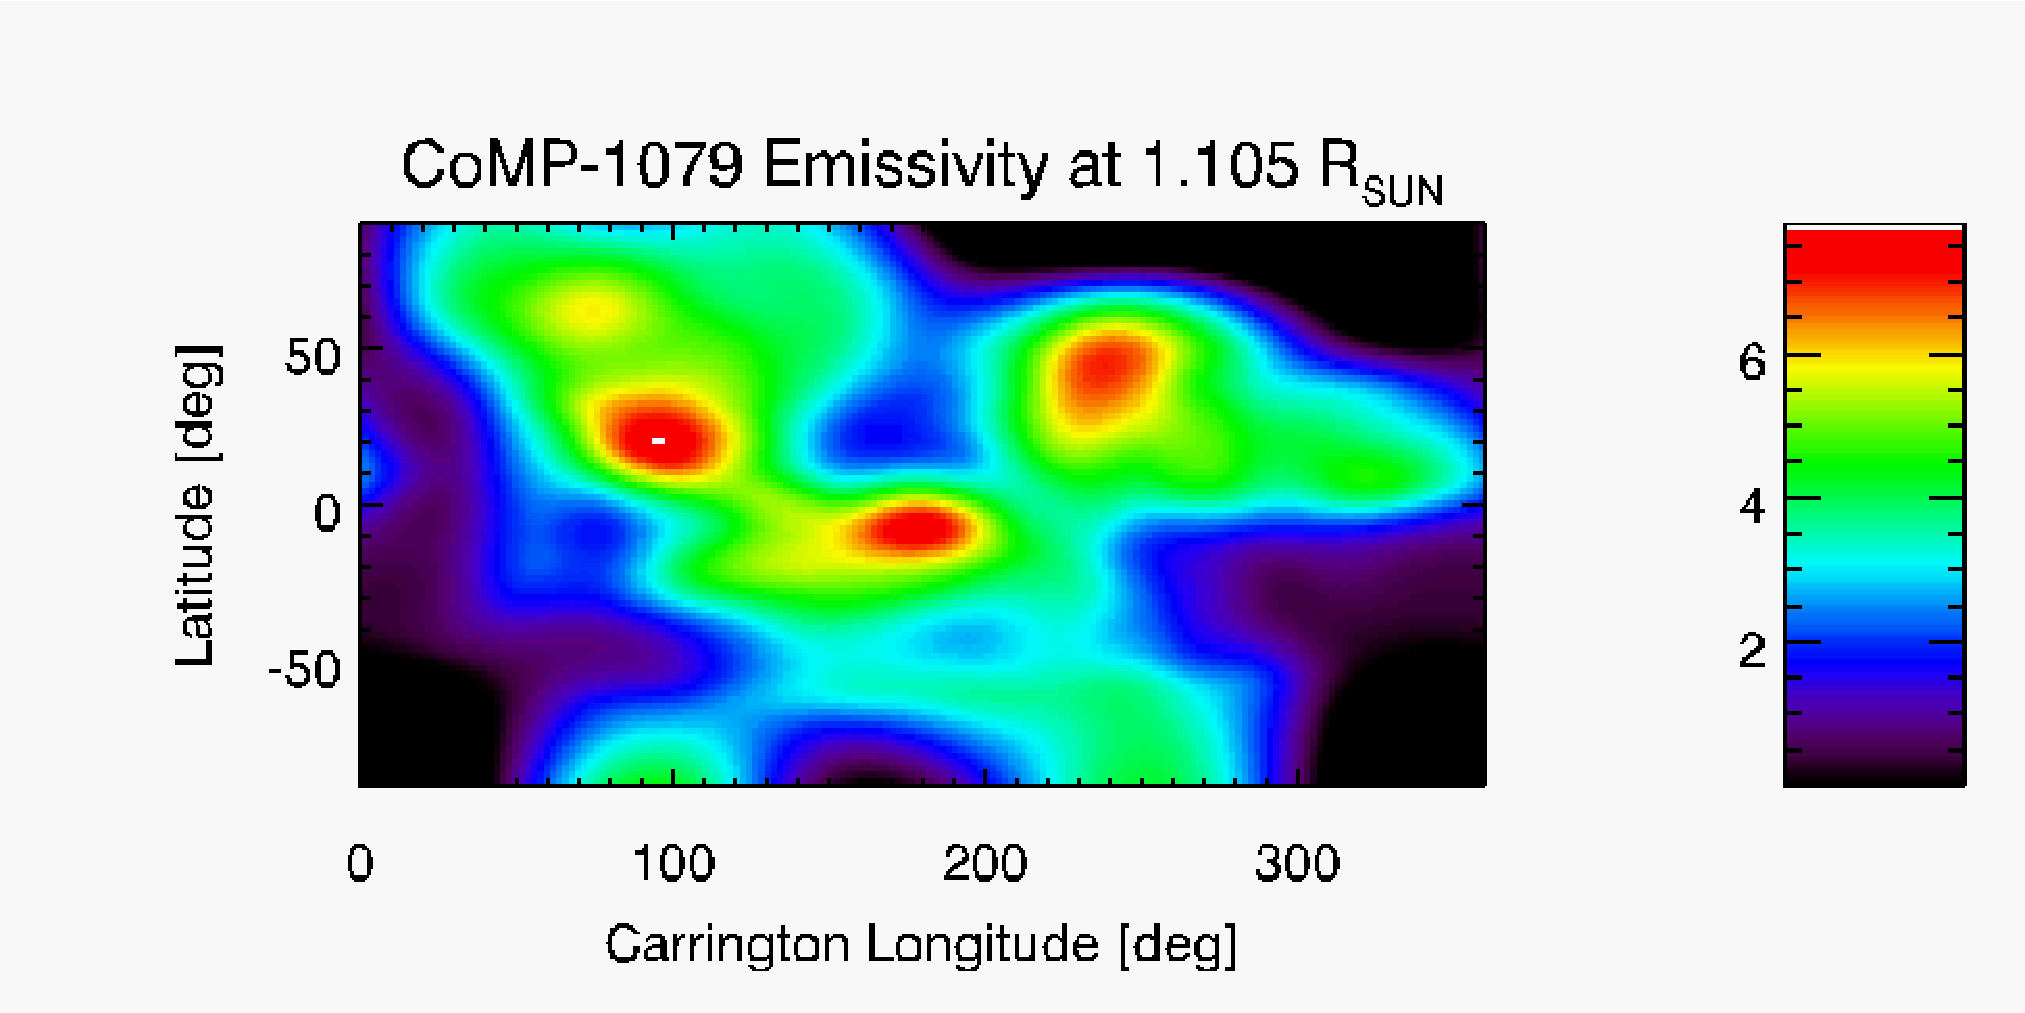
\includegraphics[width=\columnwidth]{map_x_comp1079_1105_Rsun.pdf}
\vskip 0.1cm
\azul{The time series taken by each instrument is used for an independent tomographic reconstruction.}
\end{center}
}
}
\headerbox{$N_e$: WL-tomography versus EUV-tomography}{name=KCORTom_DEMT,column=1.4,below=Tom,span=1.6}{
{\footnotesize\sf
\begin{center}
Comparison of tomographic reconstructions of $Ne$ from EUV (left) or WL (right) data\\ 
  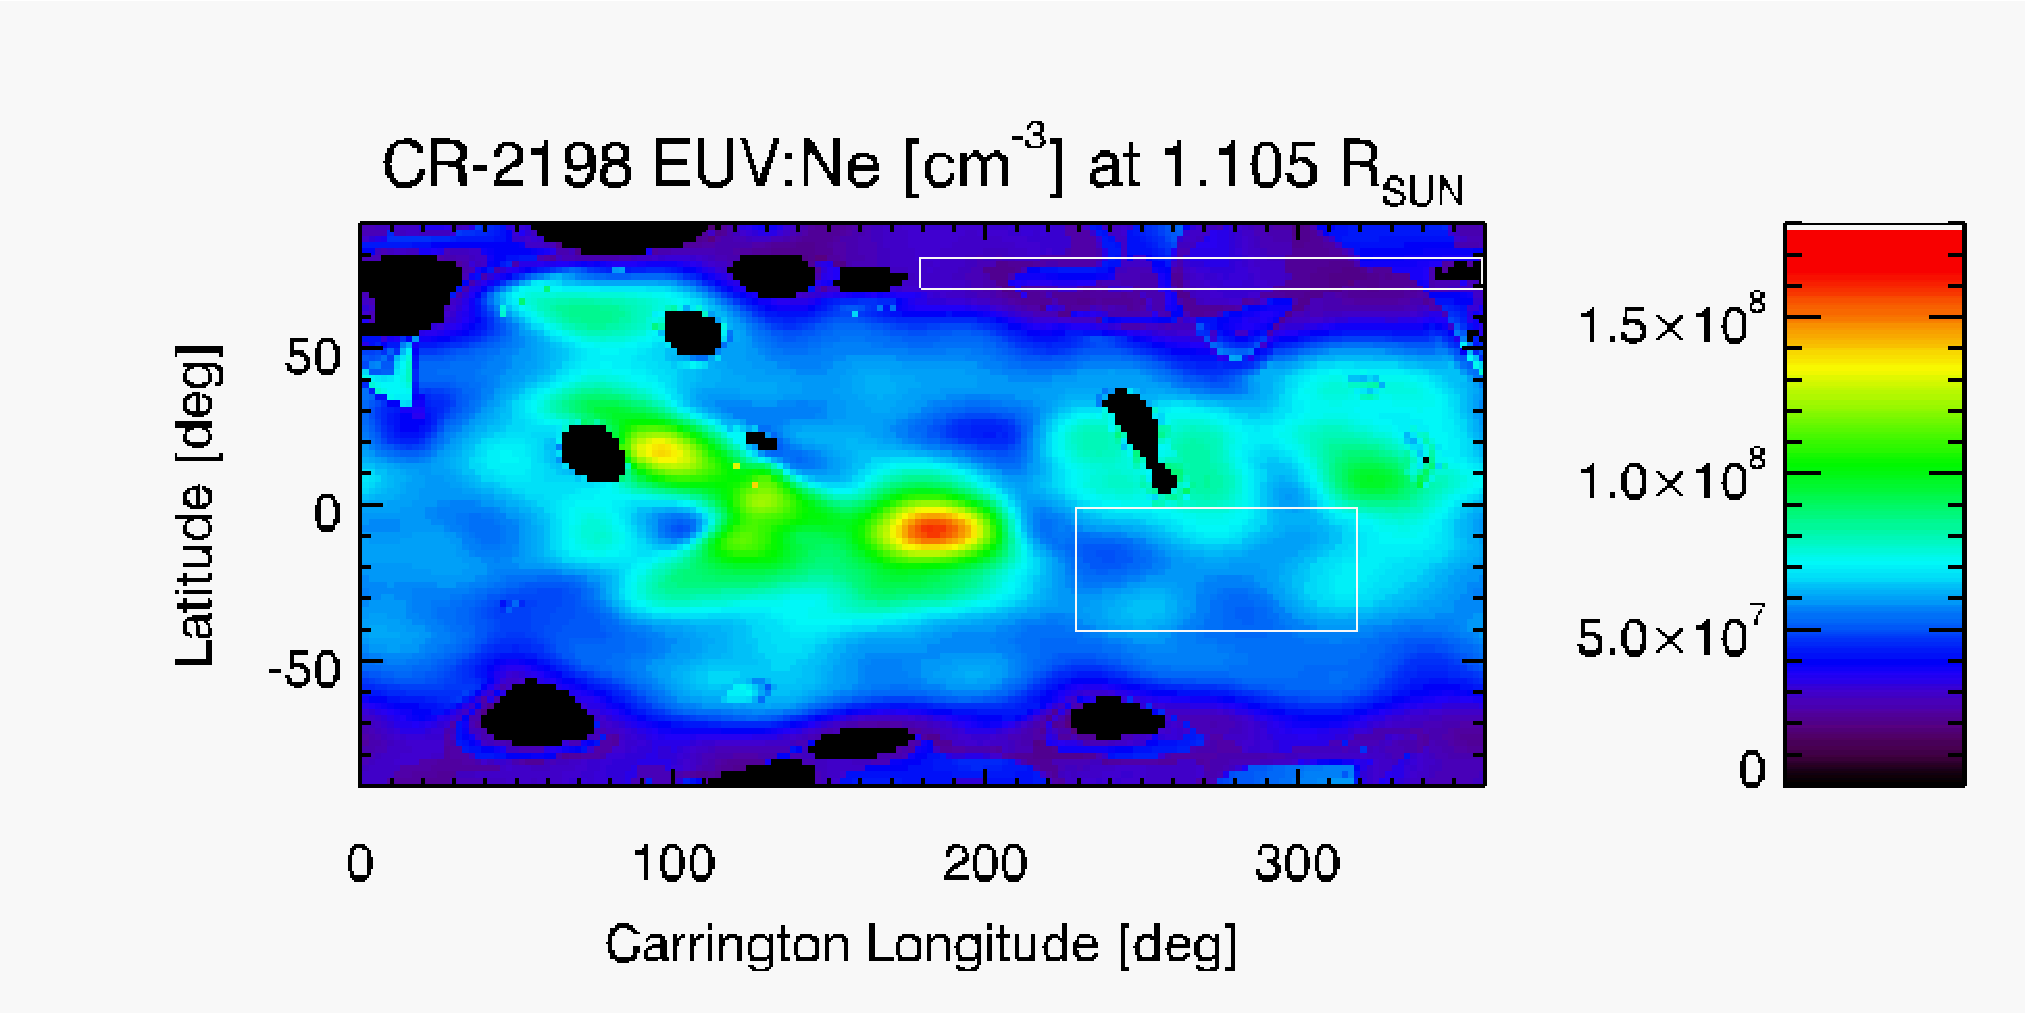
\includegraphics[width=0.45\columnwidth]{map_Ne_CR2198_DEMT-AIA_H1-L799_r3D_reduced_1105_Rsun.pdf}
  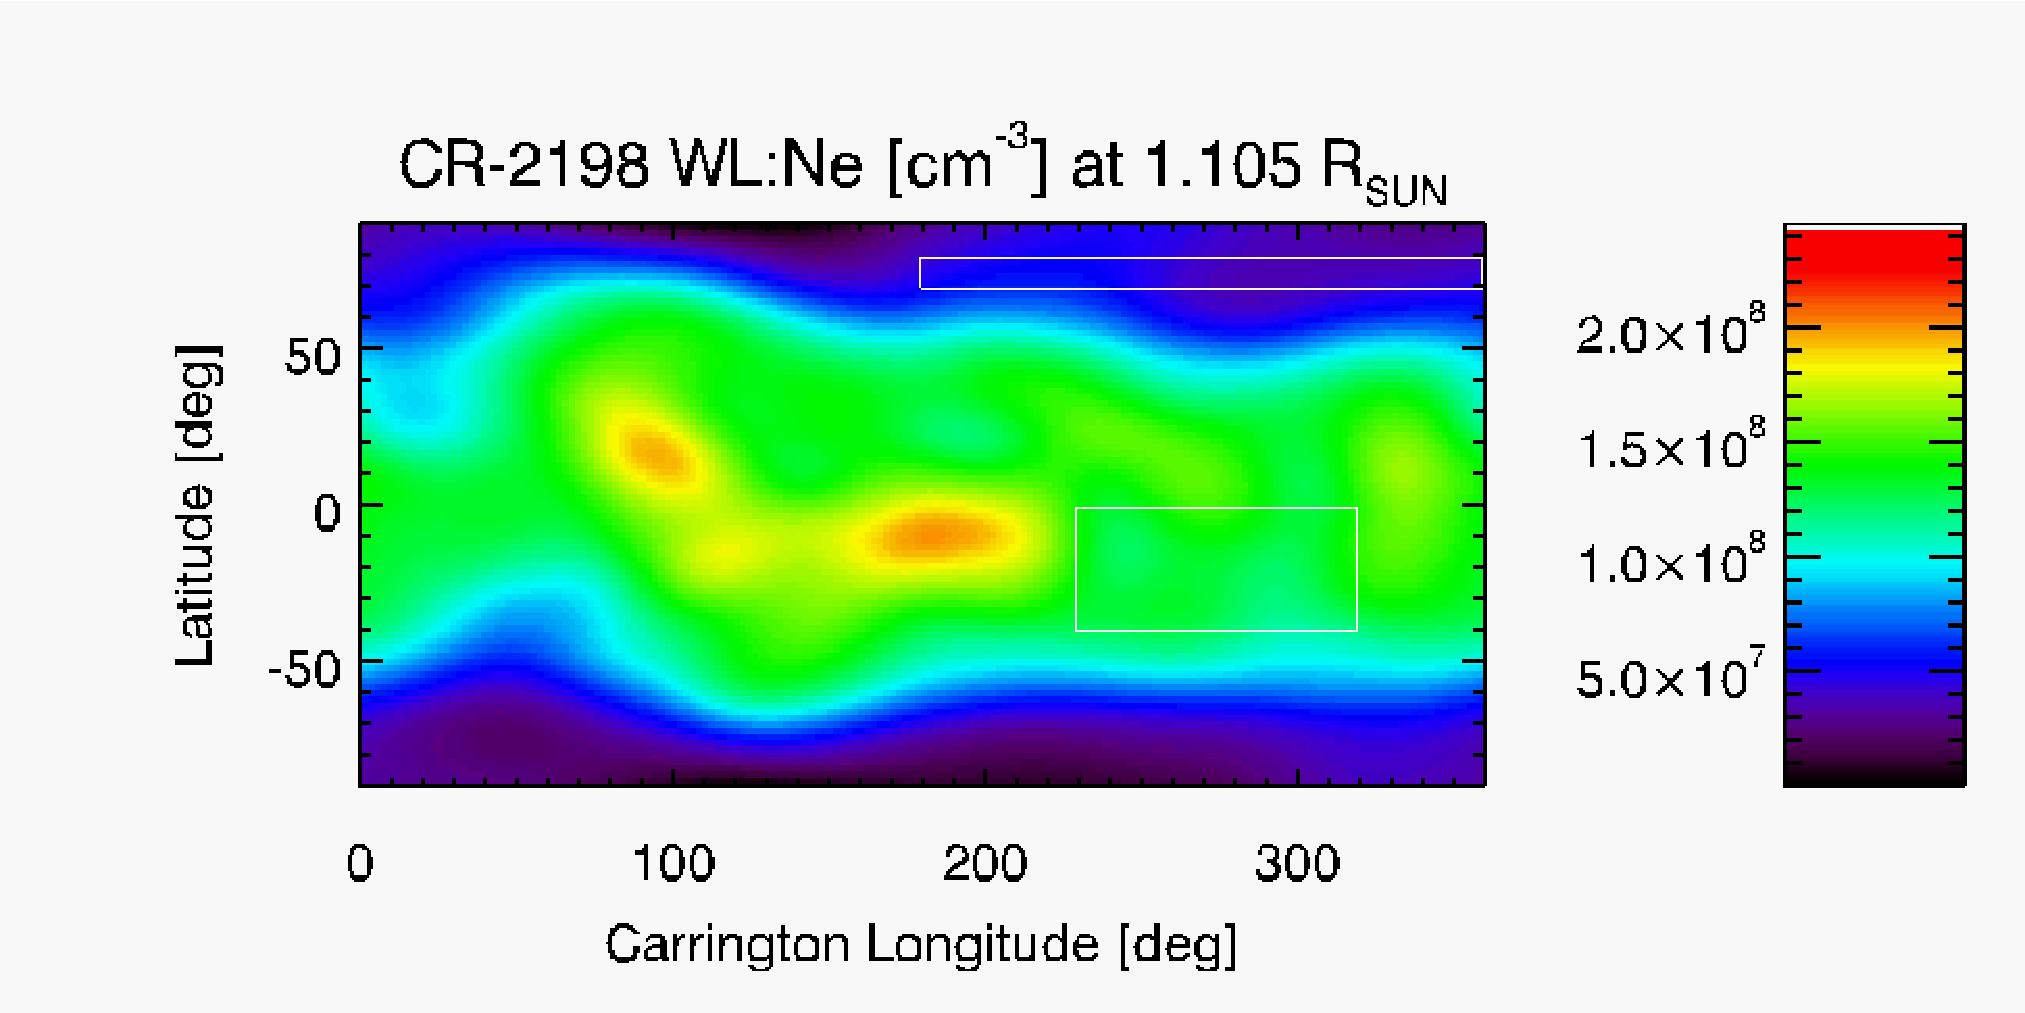
\includegraphics[width=0.45\columnwidth]{map_x_KCORCR219813imgs-reducedbf2ri105ro225_Inst_109_200_120_90_180_dropneg_r3D_l1e-4_1105_Rsun.pdf}\\
  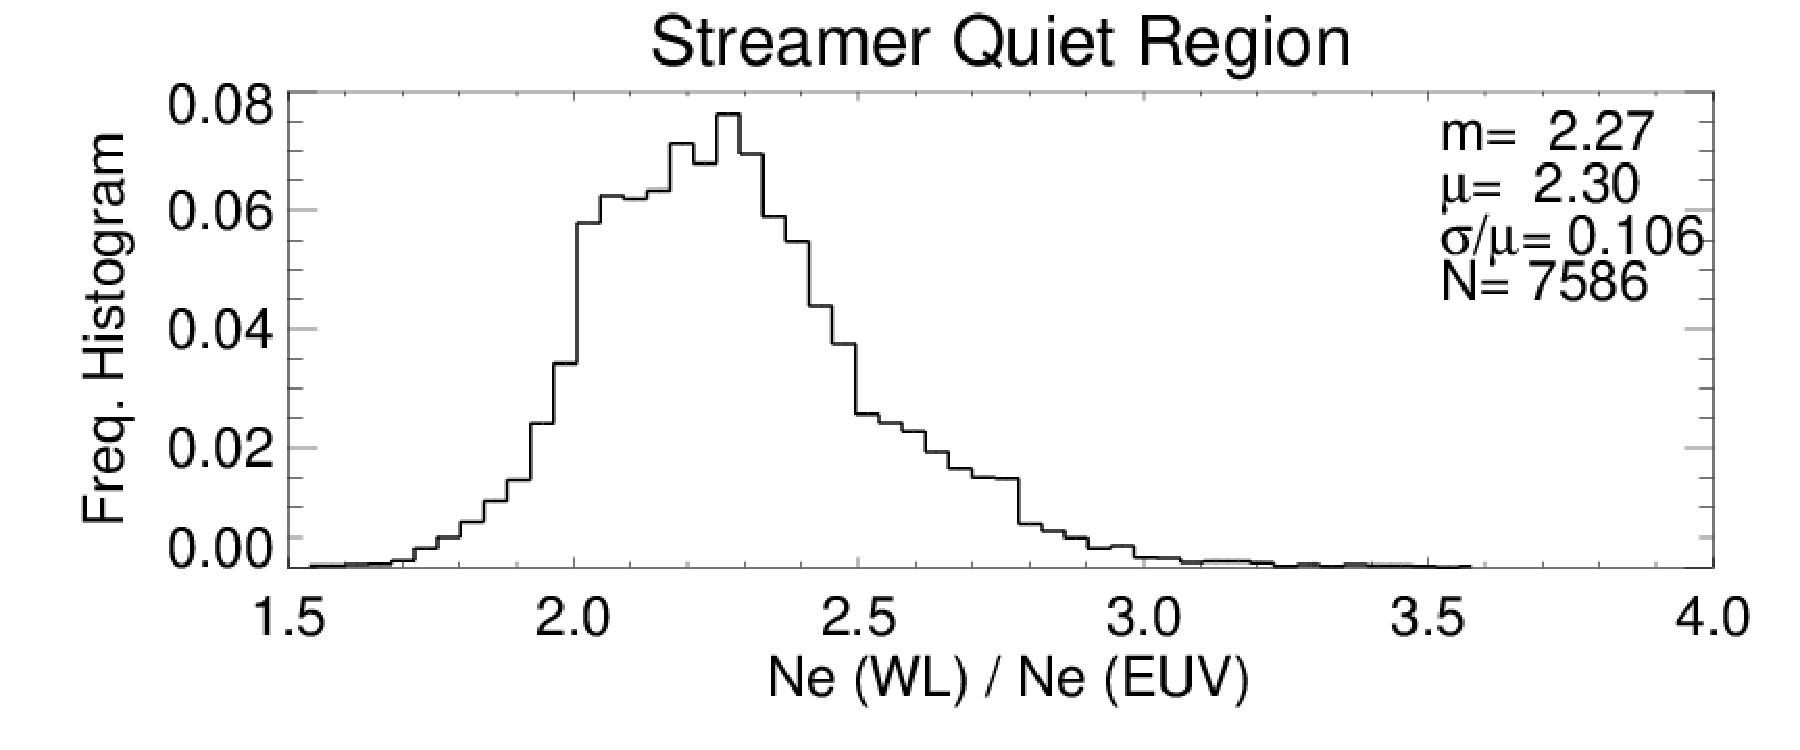
\includegraphics[width=0.37\columnwidth]{comparison_KCOR-Tom_vs_DEMT_CR2198_h_l799_reduced_kcor_1e4_newgrid-Quiet-region1_ratio_range1105-1195_Rsun.pdf}
  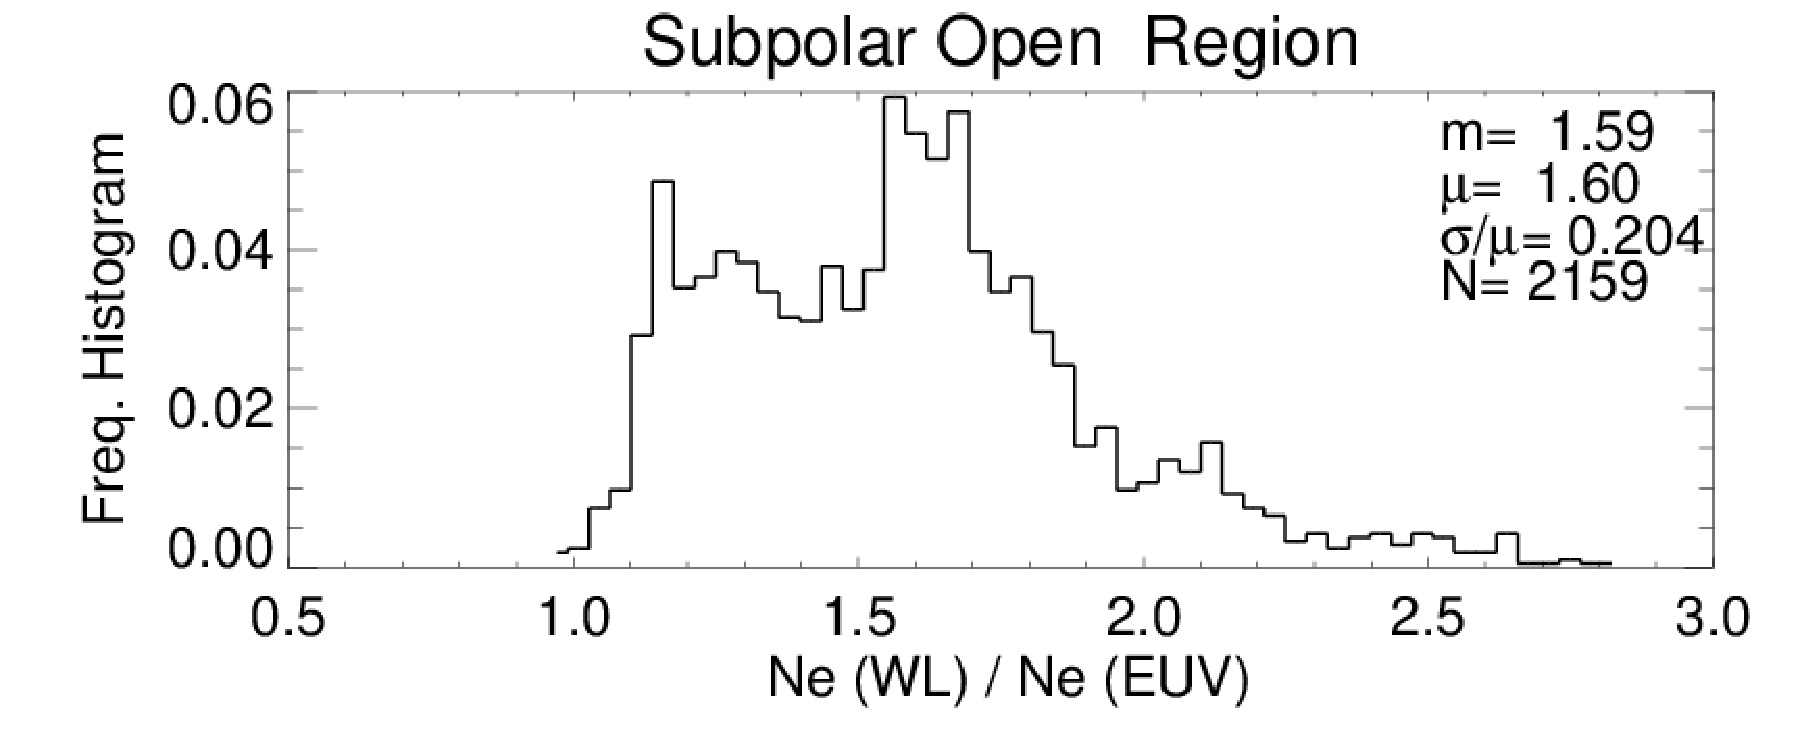
\includegraphics[width=0.37\columnwidth]{comparison_KCOR-Tom_vs_DEMT_CR2198_h_l799_reduced_kcor_1e4_newgrid-Open-region_N_ratio_range1105-1155_Rsun.pdf}\\
  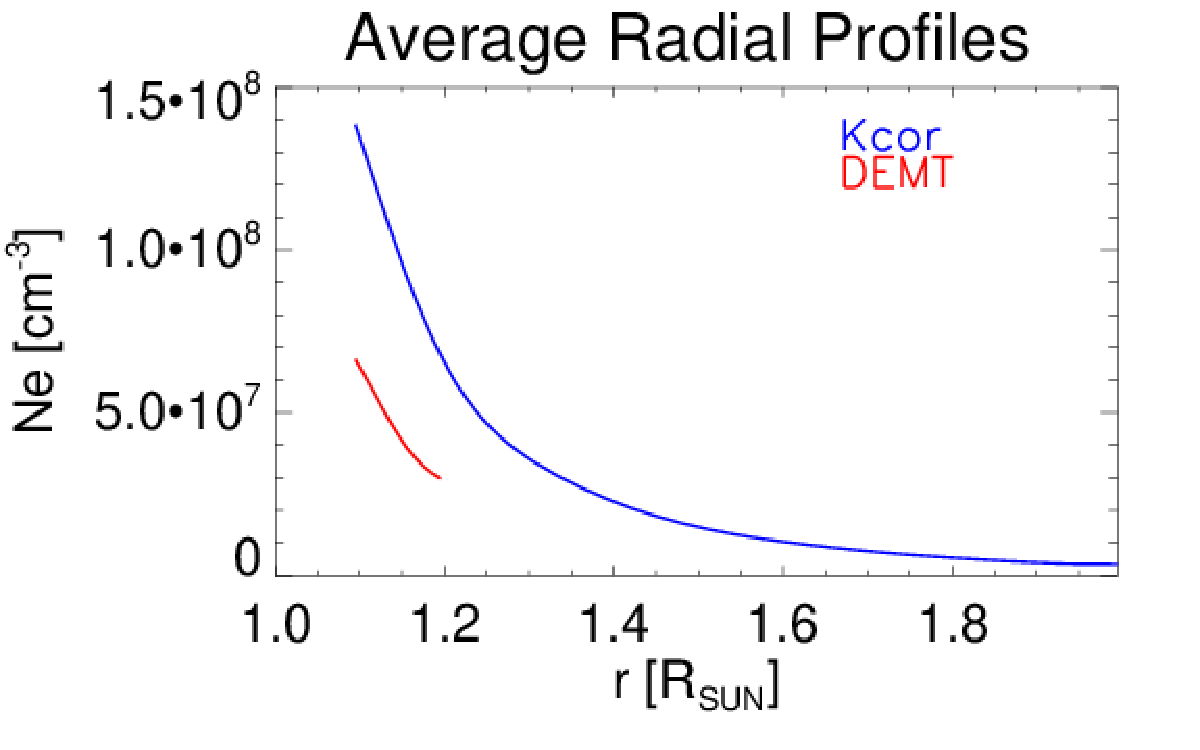
\includegraphics[width=0.37\columnwidth]{Average_Radial_Profiles_KCOR-Tom_vs_DEMT_CR2198_h_l799_reduced_kcor_1e4_newgrid-Quiet-region1.pdf}
  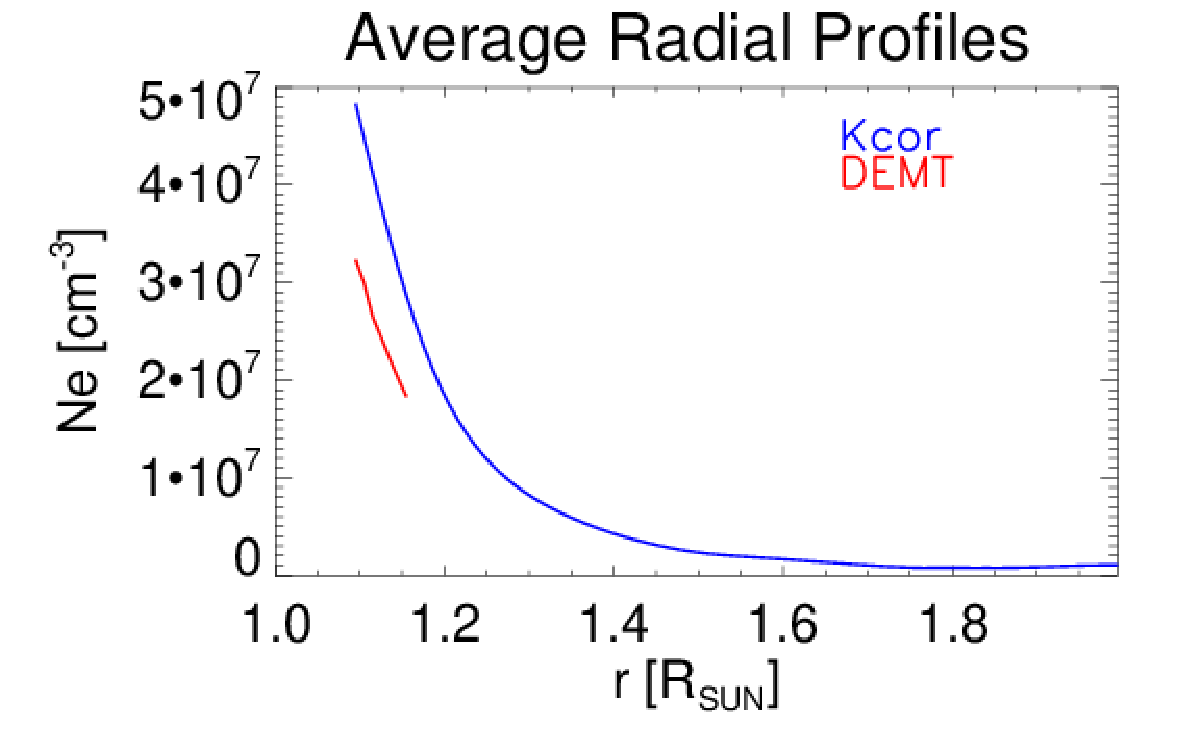
\includegraphics[width=0.37\columnwidth]{Average_Radial_Profiles_KCOR-Tom_vs_DEMT_CR2198_h_l799_reduced_kcor_1e4_newgrid-Open-region_N.pdf}
  \\
  \hrulefill
  \saltito
  Assuming that the plasma is isothermic in each tomographic voxel, the coronal irregularity factor scales as
  \azul{$X \equiv \AvgNeSQ^{(\rm{Tom-EUV})} / \left(\AvgNe^{(\rm{Tom-LB})}\right)^2 \propto 1 / \AFe$}.
  \saltito
  Assuming $\AFe$ values it is posible determine $X$. The results are inconsistent with the theory ($X>1$), suggesting that the assumptions are too simplistic.
  \saltito
  To jointly determine the values of $\AFe$ and $X$ it is necessary to consider the correlation between the distributions of $N_e$ and $T_e$. This motivates the development of a new tomographic technique.

\end{center}
}
}

\headerbox{Multi Instrument Tomography (MIT)}{name=Conclusions,column=1.4,below=KCORTom_DEMT,span=1.6}{
{\footnotesize\sf

\begin{itemize}

\item $T_e$ and $N_e$ vary within each tomographic voxel. Let us model the probability that a tiny volume of plasma has values ($T_e$, $N_e$) as: 
%\hskip 0.2cm 
\azul{$\mathcal{P} (N_e, T_e | T_m, N_m, \sigma_T, \sigma_N, q )  = \\  \frac{1}{2 \pi \sigma_T \sigma_N \sqrt{1-q^2} }  
\times \exp \left\{ \frac{-1}{2(1 - q^2)} \left[ \frac{ (T_e - T_m)^2 }{\sigma_T^2} + \frac{(N_e - N_m)^2}{\sigma_N^2}  
- \frac{2 q (T_e-T_m)(N_e - N_m)}{\sigma_T \sigma_N}   \right]  \right\}$},\\
where \azul{$N_m$} and \azul{$T_m$} are the mean electron density in the voxel, \azul{$\sigma_T$} and \azul{$\sigma_N$} are standard deviations, and \azul{$q$} is the \emph{temperature-density correlation coefficient}.   

\item
We aim at estimating the parameters \azul{$(N_m, \bc) \equiv (N_m, \AFe, T_m, \sigma_T, \sigma_N, q)$} from the joint tomographic measurements in each voxel.

\item Let a spectral synthesis model of the $M$ spectral lines and EUV band (such as CHIANTI) be represented by \azul{$s_k (\AFe, T_e, N_e)$} where \azul{$k = (1, \dots, M)$}. The $k$-\underline{th} tomographic emisivity in the computational volume element \azul{$\epsilon_k$} is given by:\\
\azul{$\epsilon_k(N_m, \bc) = \int \rd T_e \ \int \rd N_e \ s_k(\AFe, T_e, N_e) \ \mathcal{P}(T_e, N_e | N_m, T_m, \sigma_T, \sigma_N, q)$}.

\item Let us call $\by = ( y_1, \dots , y_M)$ the vector of tomographic measurements for a voxel, except for the white-light measurements of the density, which is $y_0$, not included in the vector $y$.

\item Let \azul{$\bSigma$} be the \azul{$M \times M$} uncertainty covariance matrix of the CoMP (or UCoMP) and EUV measurements. Treating all uncertainties as uncorrelated, \azul{$\bSigma$} is diagonal and the \emph{maximum likelihood estimate} of the parameter vector \azul{$\bc$} can be found in each voxel performing,\\ 
\azul{$(\hat{N}_m, \hat{\bc}) = \underset{N_m, \bc}{\mathrm{argmin}} \bigg[  \frac{ (N_m - y_0)^2}{\sigma^2_\mathrm{wl}} +  \big(\bepsilon(\bc) - \by \big)^\rT \bSigma^{-1} \big( \bepsilon(\bc) - \by \big) \, \bigg]$},
where \azul{$\bepsilon \equiv (\epsilon_1, \dots, \epsilon_M)$}.

\item Once \azul{$(\hat{N}_m, \hat{\bc})$} is found in each voxel with valid data, $X$ can be computed.

\item The technique is currently being implemented, based on the tomographic products shown here. It will be adapted to use UCoMP data once the instrument is operational.
\end{itemize}
}
}
\end{poster}
\end{document}
